\documentclass[11pt,]{article}
\usepackage{lmodern}
\usepackage{amssymb,amsmath}
\usepackage{ifxetex,ifluatex}
\usepackage{fixltx2e} % provides \textsubscript
\ifnum 0\ifxetex 1\fi\ifluatex 1\fi=0 % if pdftex
  \usepackage[T1]{fontenc}
  \usepackage[utf8]{inputenc}
\else % if luatex or xelatex
  \ifxetex
    \usepackage{mathspec}
    \usepackage{xltxtra,xunicode}
  \else
    \usepackage{fontspec}
  \fi
  \defaultfontfeatures{Mapping=tex-text,Scale=MatchLowercase}
  \newcommand{\euro}{€}
    \setmainfont{Georgia}
\fi
% use upquote if available, for straight quotes in verbatim environments
\IfFileExists{upquote.sty}{\usepackage{upquote}}{}
% use microtype if available
\IfFileExists{microtype.sty}{%
\usepackage{microtype}
\UseMicrotypeSet[protrusion]{basicmath} % disable protrusion for tt fonts
}{}
\usepackage[margin=1.0in]{geometry}
\ifxetex
  \usepackage[setpagesize=false, % page size defined by xetex
              unicode=false, % unicode breaks when used with xetex
              xetex]{hyperref}
\else
  \usepackage[unicode=true]{hyperref}
\fi
\hypersetup{breaklinks=true,
            bookmarks=true,
            pdfauthor={},
            pdftitle={},
            colorlinks=true,
            citecolor=blue,
            urlcolor=blue,
            linkcolor=magenta,
            pdfborder={0 0 0}}
\urlstyle{same}  % don't use monospace font for urls
\usepackage{graphicx,grffile}
\makeatletter
\def\maxwidth{\ifdim\Gin@nat@width>\linewidth\linewidth\else\Gin@nat@width\fi}
\def\maxheight{\ifdim\Gin@nat@height>\textheight\textheight\else\Gin@nat@height\fi}
\makeatother
% Scale images if necessary, so that they will not overflow the page
% margins by default, and it is still possible to overwrite the defaults
% using explicit options in \includegraphics[width, height, ...]{}
\setkeys{Gin}{width=\maxwidth,height=\maxheight,keepaspectratio}
\setlength{\parindent}{0pt}
\setlength{\parskip}{6pt plus 2pt minus 1pt}
\setlength{\emergencystretch}{3em}  % prevent overfull lines
\providecommand{\tightlist}{%
  \setlength{\itemsep}{0pt}\setlength{\parskip}{0pt}}
\setcounter{secnumdepth}{0}

%%% Use protect on footnotes to avoid problems with footnotes in titles
\let\rmarkdownfootnote\footnote%
\def\footnote{\protect\rmarkdownfootnote}

%%% Change title format to be more compact
\usepackage{titling}

% Create subtitle command for use in maketitle
\newcommand{\subtitle}[1]{
  \posttitle{
    \begin{center}\large#1\end{center}
    }
}

\setlength{\droptitle}{-2em}
  \title{}
  \pretitle{\vspace{\droptitle}}
  \posttitle{}
  \author{}
  \preauthor{}\postauthor{}
  \date{}
  \predate{}\postdate{}

\usepackage{booktabs}
\usepackage[final]{changes}
\usepackage[font={small},labelfont=bf,labelsep=colon]{caption}
\linespread{1.5}
\usepackage[compact]{titlesec}
\usepackage{enumitem}
\usepackage{tikz}
\def\checkmark{\tikz\fill[scale=0.4](0,.35) -- (.25,0) -- (1,.7) -- (.25,.15) -- cycle;}
\setlist{nolistsep}
\titlespacing{\section}{2pt}{*0}{*0}
\titlespacing{\subsection}{2pt}{*0}{*0}
\titlespacing{\subsubsection}{2pt}{*0}{*0}
\setlength{\parskip}{3pt}
\setremarkmarkup{(#2)}
\definechangesauthor[name={Nick Tustison}, color=red]{nt}
\definechangesauthor[name={James Stone}, color=magenta]{js}
\definechangesauthor[name={Lisa Wilde}, color=cyan]{lw}
\definechangesauthor[name={Andy Mayer}, color=green]{am}
\definechangesauthor[name={Harvey Levin}, color=blue]{hl}
\definechangesauthor[name={Brian Taylor}, color=purple]{bt}
\definechangesauthor[name={David Tate}, color=orange]{dt}

% Redefines (sub)paragraphs to behave more like sections
\ifx\paragraph\undefined\else
\let\oldparagraph\paragraph
\renewcommand{\paragraph}[1]{\oldparagraph{#1}\mbox{}}
\fi
\ifx\subparagraph\undefined\else
\let\oldsubparagraph\subparagraph
\renewcommand{\subparagraph}[1]{\oldsubparagraph{#1}\mbox{}}
\fi

\begin{document}
\maketitle

\pagenumbering{gobble}

\section{Abstract}\label{abstract}

White matter hyperintensities (WMHs) are foci of abnormal signal
intensity in white matter regions seen with magnetic resonance imaging
(MRI). WMHs are associated with normal aging and have shown prognostic
value in neurological conditions such as traumatic brain injury (TBI).
The impracticality of manually quantifying these lesions limits their
clinical utility and motivates the utilization of machine learning
techniques for automated segmentation workflows. Herein, we develop a
concatenated random forest framework with tailored features for
segmenting WMHs in a TBI cohort. The framework is provided publicly
through the Advanced Normalization Tools (ANTs) and ANTsR toolkits. MR
(3D FLAIR, T2-, and T1-weighted) images from 24 service members and
veterans scanned in the Chronic Effects of Neurotrauma Consortium's
(CENC) observational study were acquired. Manual annotations were
employed for both training and evaluation using a leave-one-out
strategy. Lesion load and overlap evaluative comparisons are
complimented by feature rankings which showcase the utility of the
concatenated approach. Our findings suggest supervised learning methods
may be applied to quantify WMHs on routine brain imaging. Paired with
correlative outcome data, supervised learning methods may allow for
identification of imaging features predictive of diagnosis and prognosis
in individual TBI patients.

\clearpage

\section{Introduction}\label{introduction}

\subsection{White matter hyperintensities in
TBI}\label{white-matter-hyperintensities-in-tbi}

White matter hyperintensities (WMHs) are foci of abnormally increased
signal intensity seen within white matter regions within the cerebrum
and brainstem on fluid attenuation inversion recovery (FLAIR) magnetic
resonance imaging (MRI) sequences. These lesions are distinguished from
prominent perivascular spaces seen on T2-weighted imaging by the lack of
fluid suppression of signal on FLAIR sequences. WMHs in the
periventricular and deep brain regions are associated with normal aging
and neurological conditions including hypertension and stroke. WMHs are
also a frequent finding following traumatic brain injury (TBI) and have
been correlated with functional outcome and injury severity in both
pediatric\textsuperscript{1,2} and adult\textsuperscript{3--6}. Further,
the regional distribution and volume of WMHs have been shown to possess
prognostic value in the TBI patient\textsuperscript{2,6--8}.
Specifically, lesion volume in corpus callosum correlates with
functional scores in the acute phase following injury, while lesion
volume in frontal lobes correlates with scores at 1 year following
injury\textsuperscript{6}. Further, volume of FLAIR lesions within the
corpus callosum, brainstem, and thalamus in patients with severe TBI
correlates with Glasgow Outcome-Extended (GOS-E)
scores\textsuperscript{4}. Additionally, in patients who are comatose
following severe TBI the regional distribution of FLAIR lesions within
the pons, midbrain, hypothalamus, basal forebrain, parietal, temporal,
occipital lobes, and insula along with the observation of grasping or
chewing behavior are associated with poor outcome\textsuperscript{7}.

Despite the above findings, outside of multiple sclerosis, WMHs are not
routinely employed as a diagnostic measure in clinical practice. Their
presence within asymptomatic patients or in association with a variety
of conditions, such as stroke, dementia, neuroinflammatory conditions,
and TBI challenge their utility in narrowing a radiological differential
diagnosis. Further, performing a comprehensive manual counting of number
and distribution of lesions in the clinical setting is simply not
practical. Despite the limited inclusion of WMH observations in routine
radiological reports, two large meta-analyses demonstrated an
association between WMHs, cognitive function, increased risk of stroke,
dementia, and death\textsuperscript{9,10}. As such, the development of
automated methods for the rapid identification and quantification of
WMHs within individual patients may allow for identification of
correlative patterns between WMH number, volume, distribution, and
disease state. Further, the development of such lesion quantification
approaches may allow for the practical inclusion of this type of
information within routine radiological practice.

\subsection{Random forests for WMH
segmentation}\label{random-forests-for-wmh-segmentation}

Machine learning and pattern recognition techniques have seen increased
application for various medical image analysis workflows (see, for
example, the annual Workshop on Machine Learning in Medical Imaging held
in conjunction with the Medical Image Computing and Computer-Aided
Intervention (MICCAI) international meeting\textsuperscript{11}).
Popular techniques such as support vector machines and neural networks
have been applied successfully to clinically relevant imaging tasks such
as supervised image segmentation (e.g.,\textsuperscript{12}) and
diagnostic prediction (e.g.,\textsuperscript{13,14}). Facilitating the
current employment of such techniques are the number of available
imaging data sets\textsuperscript{15} and the public availability of
data science packages such as SciPy\textsuperscript{16} and the R
project for statistical computing\textsuperscript{17} and their
associated extensions.

The random forests framework\textsuperscript{18} is a popular machine
learning technique that has demonstrated significant
\replaced[id=dt]{utility}{utitility} for supervised segmentation tasks
(e.g., normal human brain segmentation\textsuperscript{19}) and other
computer vision applications (e.g., human gait
detection\textsuperscript{20}). In the context of neuropathology, random
forest-based paradigms have been employed in the delineation of multiple
sclerosis lesions\textsuperscript{21}, stroke
lesions\textsuperscript{22}, and brain tumors\textsuperscript{23--26}
for both single and multi-modal acquisition protocols. Of note, these
latter random forest approaches for brain tumor segmentation have
performed well in recent international competitions
\replaced[id=dt]{established in response to the lack of objective comparisons between segmentation algorithms (i.e.,  the Multimodal Brain Tumor Segmentation (BRATS) challenge was initiated in 2012}{
In response to the lack of objective comparisons between segmentation algorithms, the Multimodal Brain Tumor Segmentation (BRATS) challenge was initiated in 2012 [@Menze:2015aa] and has continued every year since under the auspices of the MICCAI conference.}\textsuperscript{27}.

Random forests are conceptually straightforward\textsuperscript{18}.
They consist of ensembles of decision trees that are built from training
data. Once constructed, data to be classified is ``pushed'' through each
decision tree resulting in a single classification ``vote'' per tree.
These votes are then used for regression or classification of the data.
Although decision trees had been extensively studied
\deleted[id=dt]{previously}, the success of employing collections of
such weak learners for boosting machine learning performance (e.g.,
AdaBoost\textsuperscript{28,29}) influenced the similarly sytled
conglomeration of decision trees into ``forests'' with randomized node
optimization\textsuperscript{30,31}. Finally,
Breiman\textsuperscript{18} improved accuracy by random sampling of
\deleted[id=dt]{the} training data (i.e., ``bagging'') resulting in the
current random forest technique \added[id=dt]{applied here}.

In this work, we develop a concatenated random forest framework with a
tailored contextual feature image set (both spatial and intensity-based)
for segmenting \replaced[id=dt]{WMHs}{white matter hyperintensities} in
\replaced[id=dt]{a arge TBI cohort}{traumatic brain injury cohorts}.
Additionally, the entire framework is provided publicly through the
well-known open-source \added[id=lw]{Advanced Normalization Tools}
(ANTs)\footnote{\url{https://github.com/stnava/ANTs}} and
ANTsR\footnote{\url{https://github.com/stnava/ANTsR}} toolkits.
\replaced[id=dt]{Further motivating this research is the availability of several large publicly available  imaging data sets that permits testing reproducibility of this automate routine for WMH segmentation and quantification.}{Further motivating this research of this work is
the public availability of the imaging data thus permitting full reproducibility
of the results reported and discussed.}

\section{Materials and Methods}\label{materials-and-methods}

\subsection{Imaging}\label{imaging}

MR images utilized for this initial report were acquired from 24
individuals scanned at a single site involved in the Chronic Effects of
Neurotrauma Consortium's (CENC) observational study
(\added[id=nt,remark=NT: reference needed?]{see [Walker], this issue}).
Briefly, participants were Operation Enduring Freedom/ Operation Iraqi
Freedom /Operation New dawn (OEF/OIF/OND) era service members and
veterans between the ages of 18--60 who have experienced combat
situations and are between X and X (period of time) from deployment.
\added[id=js,remark={JS: Data needed.}]{The feature images consisted of subjects aged $X.X \pm X$ years (range X – X years), XX percent male, with at least one or more potential concussive events (mean = X, SD = X, range X-X).}

Images were acquired on a Philips 3.0T Ingenia system with an 8-channel
SENSE head coil (Philips Medical Systems, Best, Netherlands). 3D FLAIR
sequences were acquired with a turbo spin echo inversion recovery
sequence with the following parameters: repetition time (TR) = 4800 ms,
echo time (TE) = 325 ms, inversion time (TI) = 1650 ms; 170 sagittal
slices with a 1.2 mm slice thickness, 256 x 256 acquisition matrix, and
256 x 256 mm FOV. 3D T1-weighted sequences were acquired with a fast
field echo (FFE) sequence with the following parameters: TR = 6.8 ms, TE
= 3.2 ms, echo train length (ETL) = 240; Flip angle = 9°, 170 sagittal
slices with a 1.2 mm slice thickness, 256x240 acquisition matrix, and
256 x 256 mm FOV. In addition, 3D T2-weighted images were acquired with
a turbo spin echo sequence with the following parameters: TR = 2500 ms,
TE = 245 ms, ET: = 133; 170 sagittal slices with a 1.2 mm slice
thickness, 256 x 256 acquisition matrix, and 256 x 256 mm FOV.

\subsection{Quantitative analysis}\label{quantitative-analysis}

Crucial to these supervised segmentation approaches are the creation and
selection of ``features'' as input in conjunction with
\replaced[id=lw,remark=NT: I replaced ground-truth since it is problematic anyway]
{expertly identified structures of interest}{the ground-truth} for model
construction. For the targeted application in this work (i.e., WMHs),
regression/classification are performed at the voxelwise level. In other
words, each voxel within the region of interest is sent through the
ensemble of decision trees and receives a set of classification votes
from each tree thus permitting a regression or classification solution.
Since this procedure is performed at the voxelwise level, intensity
information alone is insufficient for good segmentation performance due
to the lack of spatial context. For example, as pointed out
in\textsuperscript{32}, higher intensities can be found at the
periventricular caps in normal subjects which often confounds automated
lesion detection algorithms. Other potential confounds include MR signal
inhomogeneity and noise. Therefore, even though machine learning and
pattern recognition techniques are extremely powerful and have
significant potential, just as crucial to outcome is the creative
construction and deployment of salient feature images which we detail
below.

\subsubsection{Feature images for WMH
segmentation}\label{feature-images-for-wmh-segmentation}

\begin{table}[!htb]
  \centering
  \begin{tabular*}{0.65\textwidth}{@{\extracolsep{\fill}} ll}
    \multicolumn{1}{c}{\textbf{Feature type}} & \multicolumn{1}{c}{\textbf{Image source}} \\
    \toprule
    \midrule
    \multicolumn{2}{c}{\textbf{Intensities}} \\
    \midrule
    normalized/preprocessed & FLAIR, T1, and T2 \\
    \midrule
    \multicolumn{2}{c}{\textbf{Symmetric template}} \\
    \midrule
    template difference & FLAIR, T1, and T2 \\
    contralateral difference & FLAIR, T1, and T2 \\
    location indices & FLAIR, T1, and T2 \\
    \midrule
    \multicolumn{2}{c}{\textbf{Segmentation probabilities}} \\
    \midrule
    $Pr$(cerebrospinal fluid) & T1 \\
    $Pr$(gray matter) & T1 \\
    $Pr$(white matter) & T1 \\
    $Pr$(deep bray matter) & T1 \\
    $Pr$(brain stem) & T1 \\
    $Pr$(cerebellum) & T1 \\
    \midrule
    \multicolumn{2}{c}{\textbf{Distance maps}} \\
    \midrule
    cerebrospinal fluid & T1 brain segmentation \\
    gray matter & T1 brain segmentation \\
    deep gray matter & T1 brain segmentation \\
    whole brain & T1 brain segmentation \\
    \midrule
    \multicolumn{2}{c}{\textbf{Neighborhood statistics}} \\
    \midrule
    mean & FLAIR, T1, and T2 \\
    standard deviation & FLAIR, T1, and T2 \\
    skewness & FLAIR, T1, and T2 \\
    \midrule
    \bottomrule
  \end{tabular*}
 \label{table:indices}
 \caption{List of feature images used for Stage 1 of the proposed white matter
          hyperintensity segmentation framework.}
\end{table}




Supervised methodologies are uniquely characterized, in part, by the
feature images that are used to identify the regions of interest. In
Table 1, we provide a list and basic categorization of the feature
images used for the initial (i.e., Stage 1---more on the use of multiple
random forest stages below) segmentation of the WMHs. In addition Figure
1 provides a representation of a set of feature images for a single
subject analyzed in this work. Note that in this work we categorize the
brain parenchyma with seven labels:

\begin{itemize}
\tightlist
\item
  cerebrospinal fluid (label 1),
\item
  gray matter (label 2),
\item
  white matter (label 3),
\item
  deep gray matter (label 4),
\item
  brain stem (label 5),
\item
  cerebellum (label 6), and
\item
  white matter hyperintensities (label 7).
\end{itemize}

\begin{figure}[htbp]
\centering
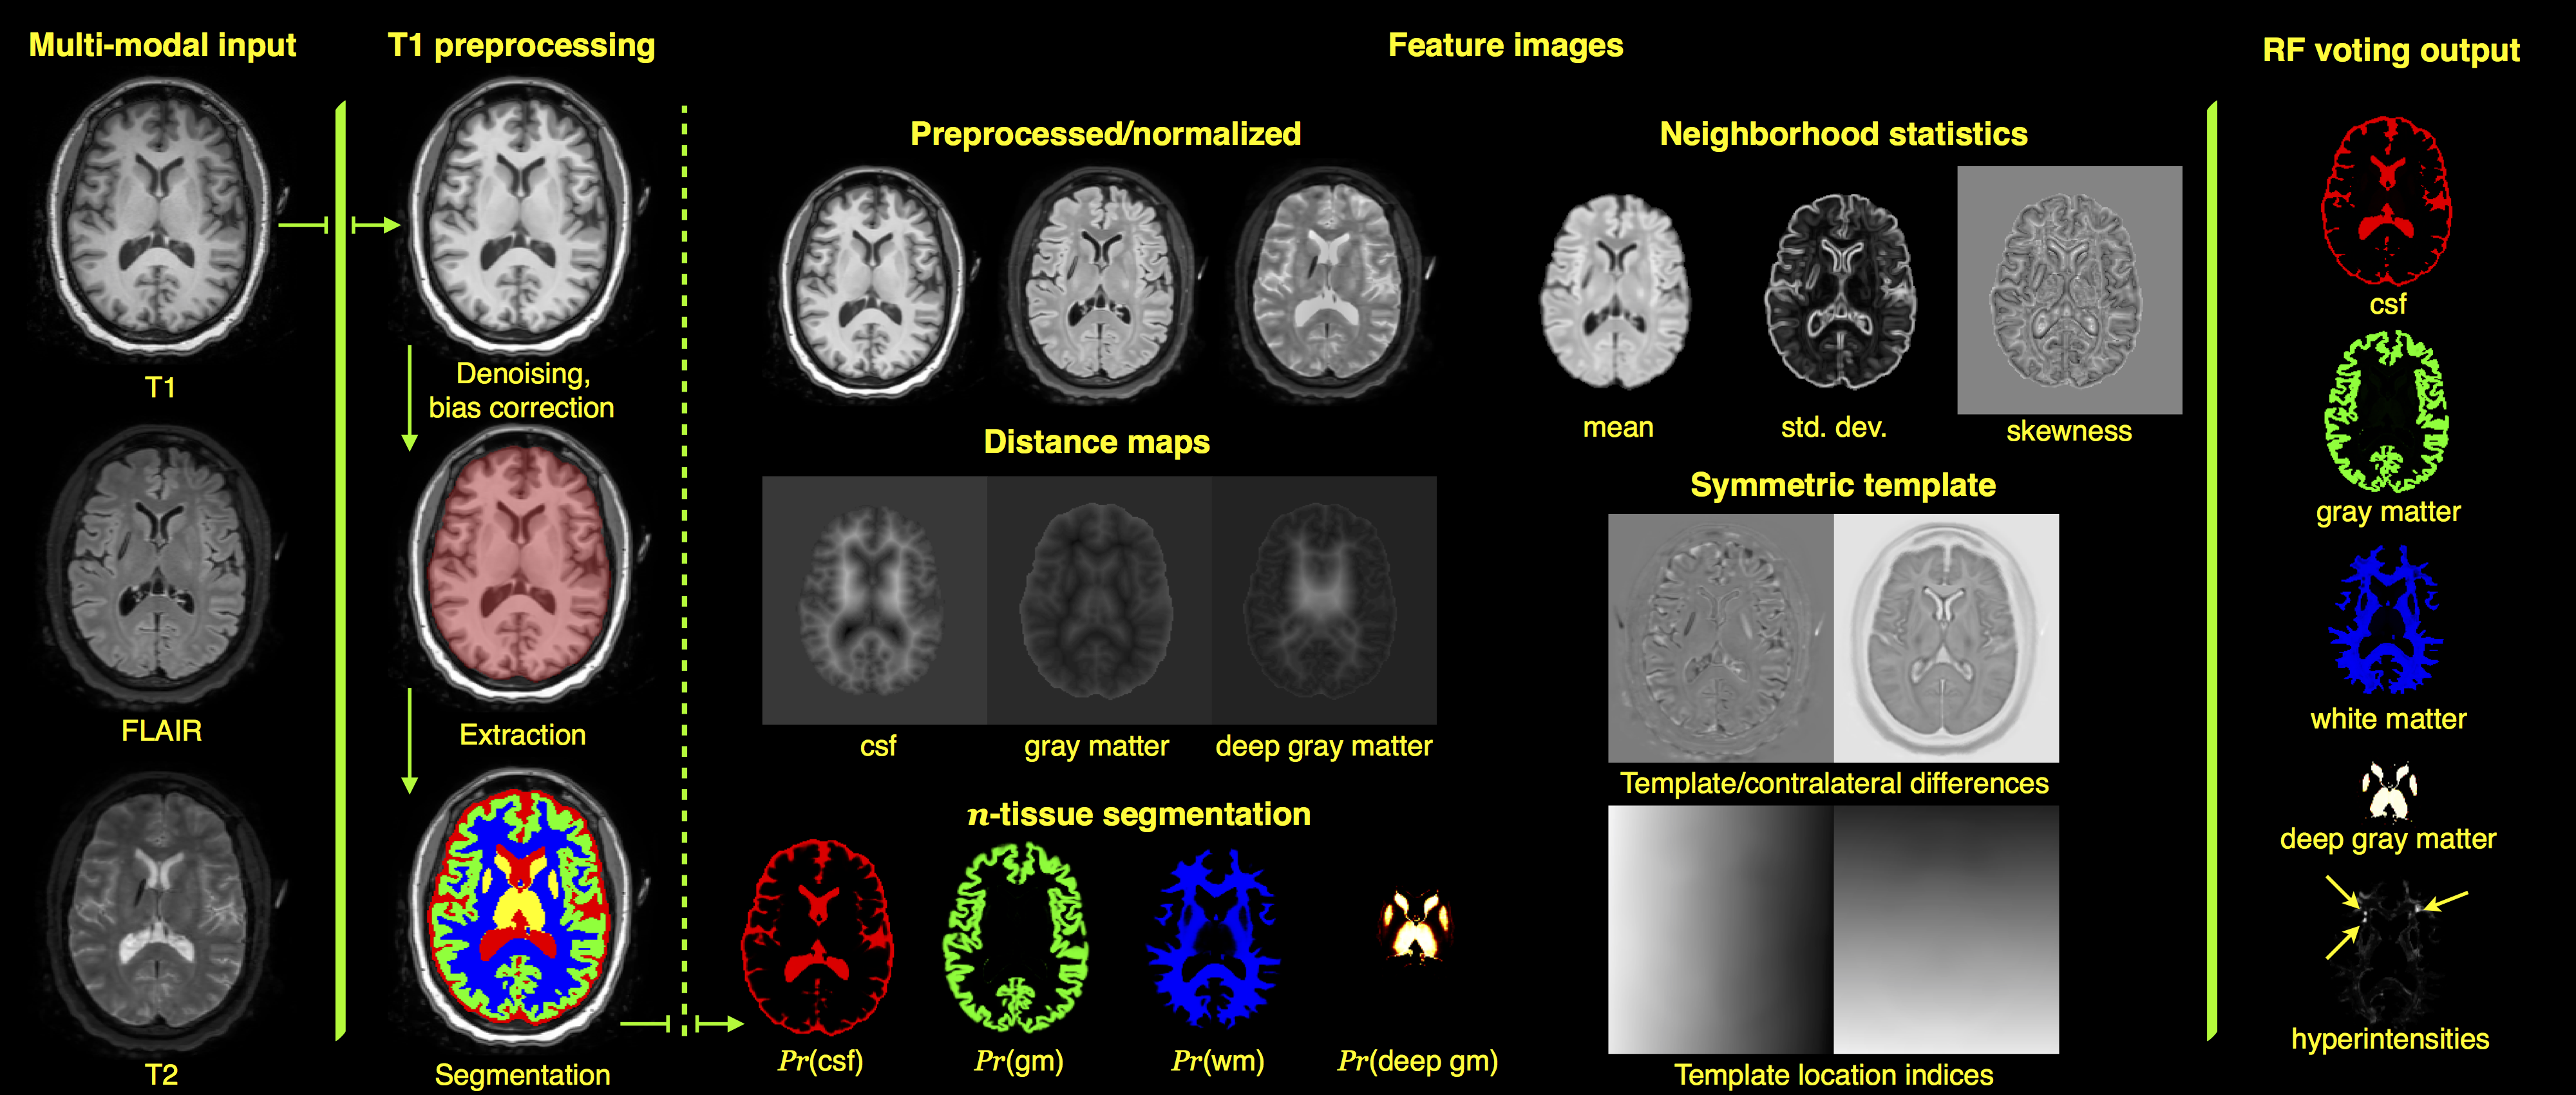
\includegraphics{Figures/featureImages.png}
\caption{Representation of Stage 1 feature images for subject 01C1019.
The FLAIR, T1-, and T2-weighted images are
\added[id=am,remark=NT: no need for 12 dof for
intra-subject normalization]{rigidly} pre-aligned\textsuperscript{33} to
the space of the T1 image. The three modality images are then
preprocessed (N4 bias correction\textsuperscript{34} and adaptive
denoising\textsuperscript{35}) followed by application of standard ANTs
brain extraction and \(n\)-tissue segmentation protocols using the MMRR
symmetric template and corresponding priors\textsuperscript{36} applied
to the T1 image. The feature images are then generated for voxelwise
input to the RF model which results in the voting maps illustrated on
the right. This gives a probabilistic classification of tissue type. Not
shown are the probability and voting images for the brain stem and
cerebellum.}
\end{figure}

As mentioned previously, input for each subject comprises FLAIR, T1-,
and T2-weighted acquisitions. The FLAIR and T2 images are rigidly
registered to the T1 image using the open-source Advanced Normalization
Tools (ANTs)\textsuperscript{33}. The aligned images are then
preprocessed using the denoising algorithm of\textsuperscript{35}
followed by N4 bias correction\textsuperscript{34} which are then
normalized to the intensity range \([0,1]\). Although we could have used
an alternative intensity standardization algorithm
(e.g.,\textsuperscript{37}), we found that a simple linear rescaling
produced better results similar
\added[id=dt]{to previous work}\textsuperscript{26}.

\begin{figure}[htbp]
\centering
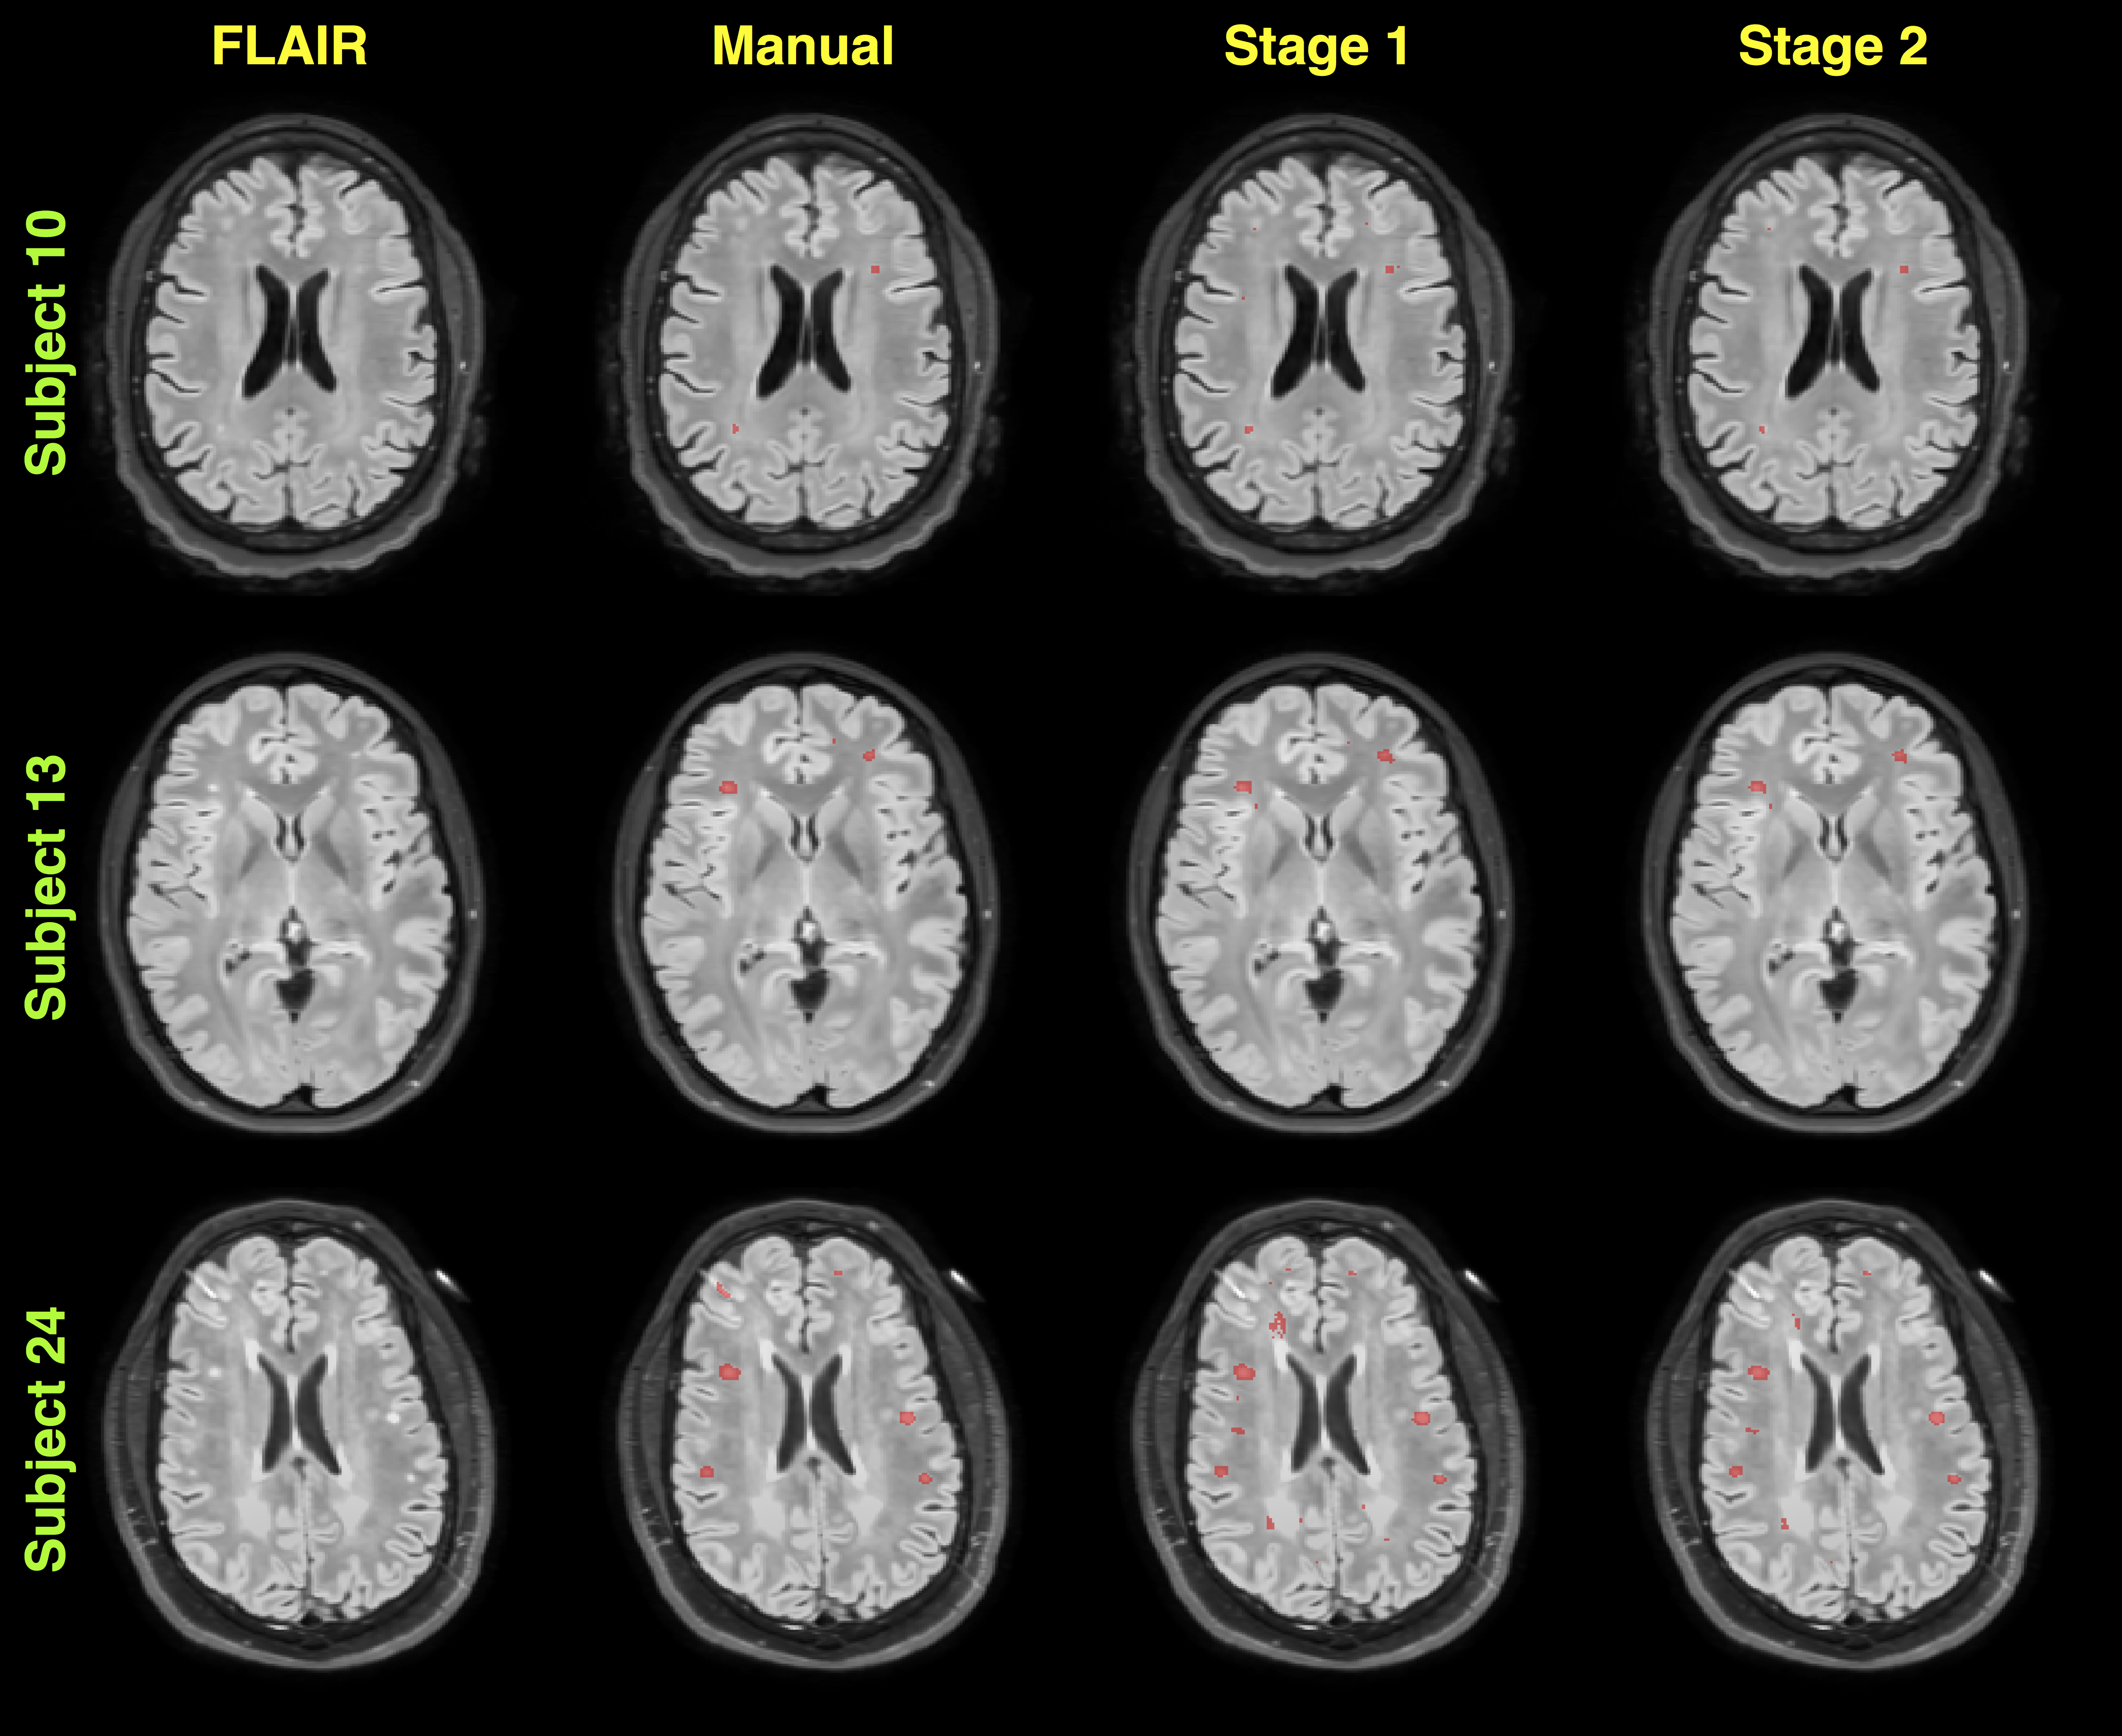
\includegraphics{Figures/sampleResults.png}
\caption{Sample FLAIR acquisition image slices showing both manual and
random forest segmentations for both stages obtained during the
leave-one-out evaluation. Manual segmentations were performed by one of
the authors and provided the ground truth WMH labels for training the
random forest models.}
\end{figure}

The T1 image is then processed via the ANTs brain extraction and normal
tissue segmentation (i.e., the pathology is discounted which is a fairly
safe assumption for the T1 image) protocols as part of the cortical
thickness pipeline described in\textsuperscript{36}.
\added[id=hl]{This protocol involves preprocessing using N4 bias correction followed by a template-based strategy for brain extraction.  Once the
brain has been extracted, we apply a Bayesian-based segmentation algorithm
with a template-based prior probability strategy to segment the
parenchymal tissue types.  The result is} a mask delineating the brain
parenchyma and probabilistic estimates of the
\replaced[id=dt]{CSF}{cerebrospinal fluid (csf)}, gray matter, white
matter, deep gray matter, brain stem, and cerebellum. These provide the
expertly annotated labels for the first six tissue labels given above.
The \replaced[id=dt]{WMHs}{white matter hyperintensities} were manually
identified by one of the authors (J. R. S.) using the ITK-SNAP
tool\textsuperscript{38}. Segmentation is performed using the ANTs
Atropos tool\textsuperscript{39} and multi-model optimal symmetric
shape/intensity templates\textsuperscript{26} created from the public
MMRR data set\textsuperscript{40} (cf Figure 3).

\begin{figure}[htbp]
\centering
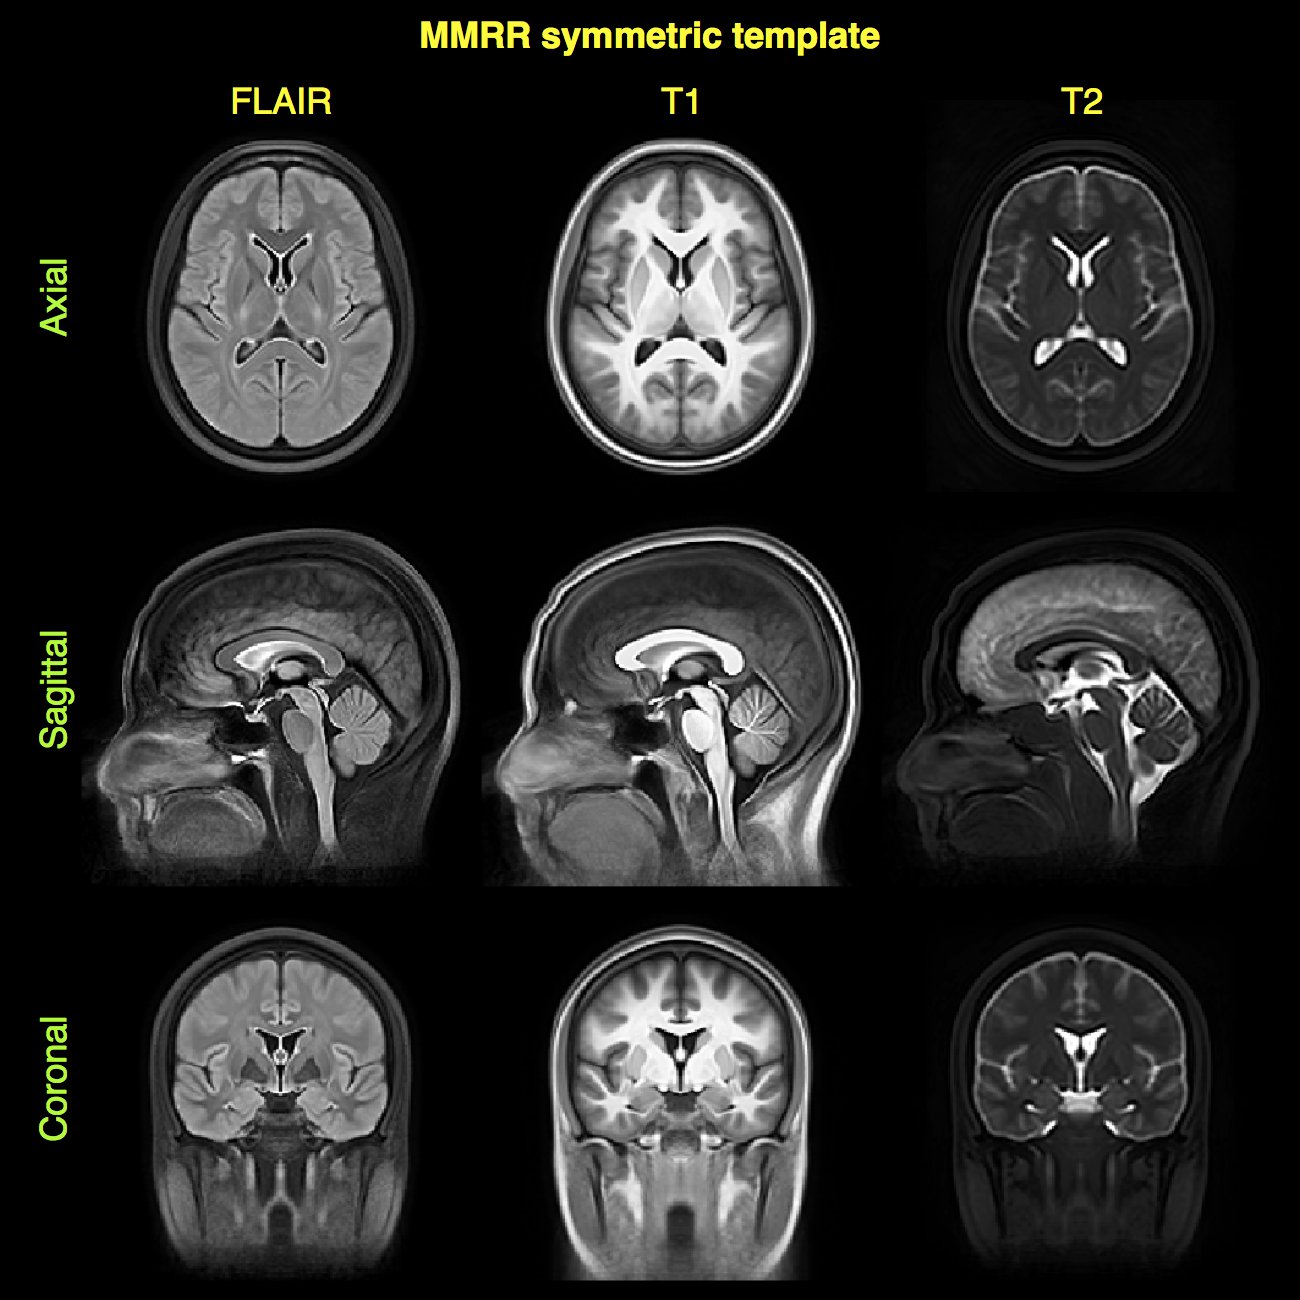
\includegraphics{Figures/MMRR.png}
\caption{Canonical views of the mutlivariate, bilaterally symmetric
template constructed from the MMRR data set\textsuperscript{40} (only
shown are the FLAIR, T1, and T2 modalities--- the components relevant
for this work). Template construction is detailed
in\textsuperscript{26}. These images are important for specific
intensity-based features.}
\end{figure}

To model the intensity information the first set of images simply
includes the preprocessed and normalized intensity FLAIR, T1, and T2
image voxel values. We also calculate a set of neighborhood statistics
(mean, standard deviation, and skewness) feature images using a
\added[id=am]{Manhattan} radius of one voxel
\added[id=nt]{given the typical size
of individual WMHs}. For each of the normalized images, we calculate the
difference in intensities with the corresponding warped template
component. Previous success in the international brain tumor
segmentation competition\textsuperscript{27} was based on an important
set of intensity features that were created from multi-modal templates
mentioned previously\textsuperscript{26}
\added[id=nt]{and listed in Table 1}. We employ the same strategy here.
For example, the template difference feature image for the FLAIR image,
\(S_{FLAIR}\) is calculated as:

\[S_{FLAIR} - T_{FLAIR}\left(\phi_b^{-1}\right)\]

where \(\phi_b: S \leftrightarrow \underset{b}{\leftrightsquigarrow} T\)
is the transform which maps from the individual subject space to the
template space and \(T_{FLAIR}\) is the FLAIR template component. Also,
to take advantage of the
\added[id=hl,remark=NT:  we are using the gross bilateral symmetry of the brain in an analogous sense that if we know the left eye location and color then we can accurately predict the location and color of the right eye even though a particular face might not be exactly symmetric]{gross}
bilateral symmetry of the normal brain (in terms of both shape and
intensity), and the fact that
\replaced[id=bt]{WMHs do not generally manifest symmetrically across hemispheres}{the presence of WMHs violates that assumption},
we use the symmetric templates to compute the contralateral intensity
differences as an additional intensity feature. For the FLAIR component,
this contralateral difference image is calculated from

\[S_{FLAIR} - S_{FLAIR}\left(\phi_b^{-1}\left(\phi_R\left(\phi_b\right)\right)\right)\]

where \(\phi_R\) denotes a horizontal reflection perpendicular to the
mid-sagittal plane of the symmetric template.

The segmentation probability images described above are used as feature
images to provide a spatial context for the random forest model
prediction step. Additional spatial contextual feature images include
the distance maps\textsuperscript{41} based on the csf, gray matter, and
deep gray matter images. These latter images are intended to help
distinguish white matter hyperintensities from false positives induced
by the partial voluming at the gray/white matter interface. A third set
of images are based on the voxel location within the space of the
template. The T1 image of the subject is registered to the T1 template
component using a B-spline variant\textsuperscript{42} of the well-known
ANTs Symmetric Normalization (SyN) algorithm\textsuperscript{43}. Since
the inverse transform is also derived as part of the registration
process, we can warp the voxel index locations back to the space of the
individual subject
\replaced[id=nt]{which motivates similar work by others}{
Note that this is similar in motivation to the work
of}\textsuperscript{44}. However, this previous work lacks the
normalization to the standard coordinate system provided by the template
to dramatically improve spatial specificity across all subjects.

\subsubsection{Stacked (concatenated) random forests for improved
segmentation
performance}\label{stacked-concatenated-random-forests-for-improved-segmentation-performance}

In previous brain tumor segmentation work\textsuperscript{26}, it was
demonstrated that a concatenated supervised approach, whereby the
prediction output from the first random forest model serves as partial
input for a second random forest model, can significantly improve
segmentation performance. We do the same thing for the work described
here
\added[id=lw]{where we employ two stacked random forests (or two "stages")}.
The Stage 1 feature images of the training data (as described
previously) are used to construct the Stage 1 model. The training data
Stage 1 features are then used to produce the voxelwise
\added[id=lw]{"voting maps" (i.e., the classification count of each decision tree for each tissue label)}
via the Stage 1 random forest model. All the Stage 1 features plus the
Stage 1 voting maps are used as input to the Stage 2 model. In addition,
we use the Stage 1 voting maps as tissue priors
\added[id=lw]{(i.e., probabilistic estimates of the tissue spatial locations)}
for a second application of the Atropos maximum aposteriori algorithm
with an additional Markov Random Field spatial prior
(MAP-MRF)\textsuperscript{39}. However, for the second stage we use all
three aligned preprocessed images for a multivariate segmentation. The
resulting seven posterior probability images constitute a third
additional feature image set for Stage 2.

\subsubsection{Code and data
availability}\label{code-and-data-availability}

As pointed out in a recent comprehensive multiple sclerosis lesion
segmentation review\textsuperscript{45}, although the number of
algorithms reported in the literature is quite extensive, there were
only four publicly available segmentation algorithms at the time of
writing \added[id=am]{this article}.
\replaced[id=dt]{In contrast to the current work,}{of which} none are
based on supervised learning. As we did for our brain tumor segmentation
algorithm\textsuperscript{26}, all of the code described in this work is
publicly available through the open-source ANTs/ANTsR toolkits. Through
ANTsR (an add-on toolkit which, in part, bridges ANTs and the R
statistical project) we use the \texttt{randomForest}
package\textsuperscript{46} using the default settings with 2000 trees
per model and 500 randomly selected samples per label per image.
\added[id=bt]{Note that we saw little variation in performance when these parameters were changed (i.e. up to 1000 random samples and as little as 1000 trees) which is consistent with our previous experience.}

In addition, similar to our previous offering,\footnote{\url{https://github.com/ntustison/ANTsAndArboles}}
we plan on creating a self-encapsulated example to showcase the proposed
methodology. The fact that the data will also be made available through
the
\replaced[id=lw]{Federal Interagency Traumatic Brain Injury Research (FITBIR)}{FITBIR}
repository along with the manual labelings will facilitate
reproducibility on the part of the reader as well as any interest in
extending the proposed framework to other data sets.

\subsubsection{Evaluation protocol
overview}\label{evaluation-protocol-overview}

In order to evaluate the protocol described, we performed a
leave-one-out evaluation using the data acquired from the 24 subjects
described above. Initial processing included the creation of all Stage 1
feature images for all subjects. The initial brain segmentation of each
T1 image and the manual white matter hyperintensity tracings were
combined to provide the truth labels for the training data. The
``truth'' labels are the seven anatomical regions given above.

The leave-one-out procedure is as follows:

\begin{itemize}
\tightlist
\item
  Create Stage 1 feature images for all 24 subjects.
\item
  For each of the 24 subjects:

  \begin{itemize}
  \tightlist
  \item
    sequester the current subject and corresponding feature images.
  \item
    construct the Stage 1 random forest model from the remaining 23
    subjects.
  \item
    apply the Stage 1 random forest model to the feature images of the
    23 training subjects.
  \item
    the previous step produces the Stage 1 voting maps for all seven
    labels.
  \item
    for each of the 23 subjects, perform a Bayesian-based segmentation
    with an MRF spatial prior using the seven voting maps are used as
    additional tissue priors.
  \item
    construct the Stage 2 random forest model from all the Stage 1
    feature images, seven voting maps, and seven posterior probability
    maps from the previous step.
  \item
    send the sequestered subject through the random forest models for
    both stages.
  \item
    compare the final results with the manually-defined white matter
    hyperintensity regions.
  \end{itemize}
\end{itemize}

\section{Results}\label{results}

\subsection{Ranking feature
importance}\label{ranking-feature-importance}

After performing the leave-one-out
evaluation\deleted[id=dt]{described at the end of the previous section},
we calculated the \texttt{MeanDecreaseAccuracy} feature values for each
of the 24 subjects \(\times\) 2 models per subject \(=48\) total models.
This measure (per feature, per model) is calculated during the
out-of-bag phase of the random forest model construction and quantifies
the decrease in prediction accuracy from omitting the specified feature.
In other words, this quantity helps determine the importance of a
particular feature and, although we save such efforts for future work,
this information provides us with guidance for future feature pruning
and/or additions.

\begin{figure}[htbp]
\centering
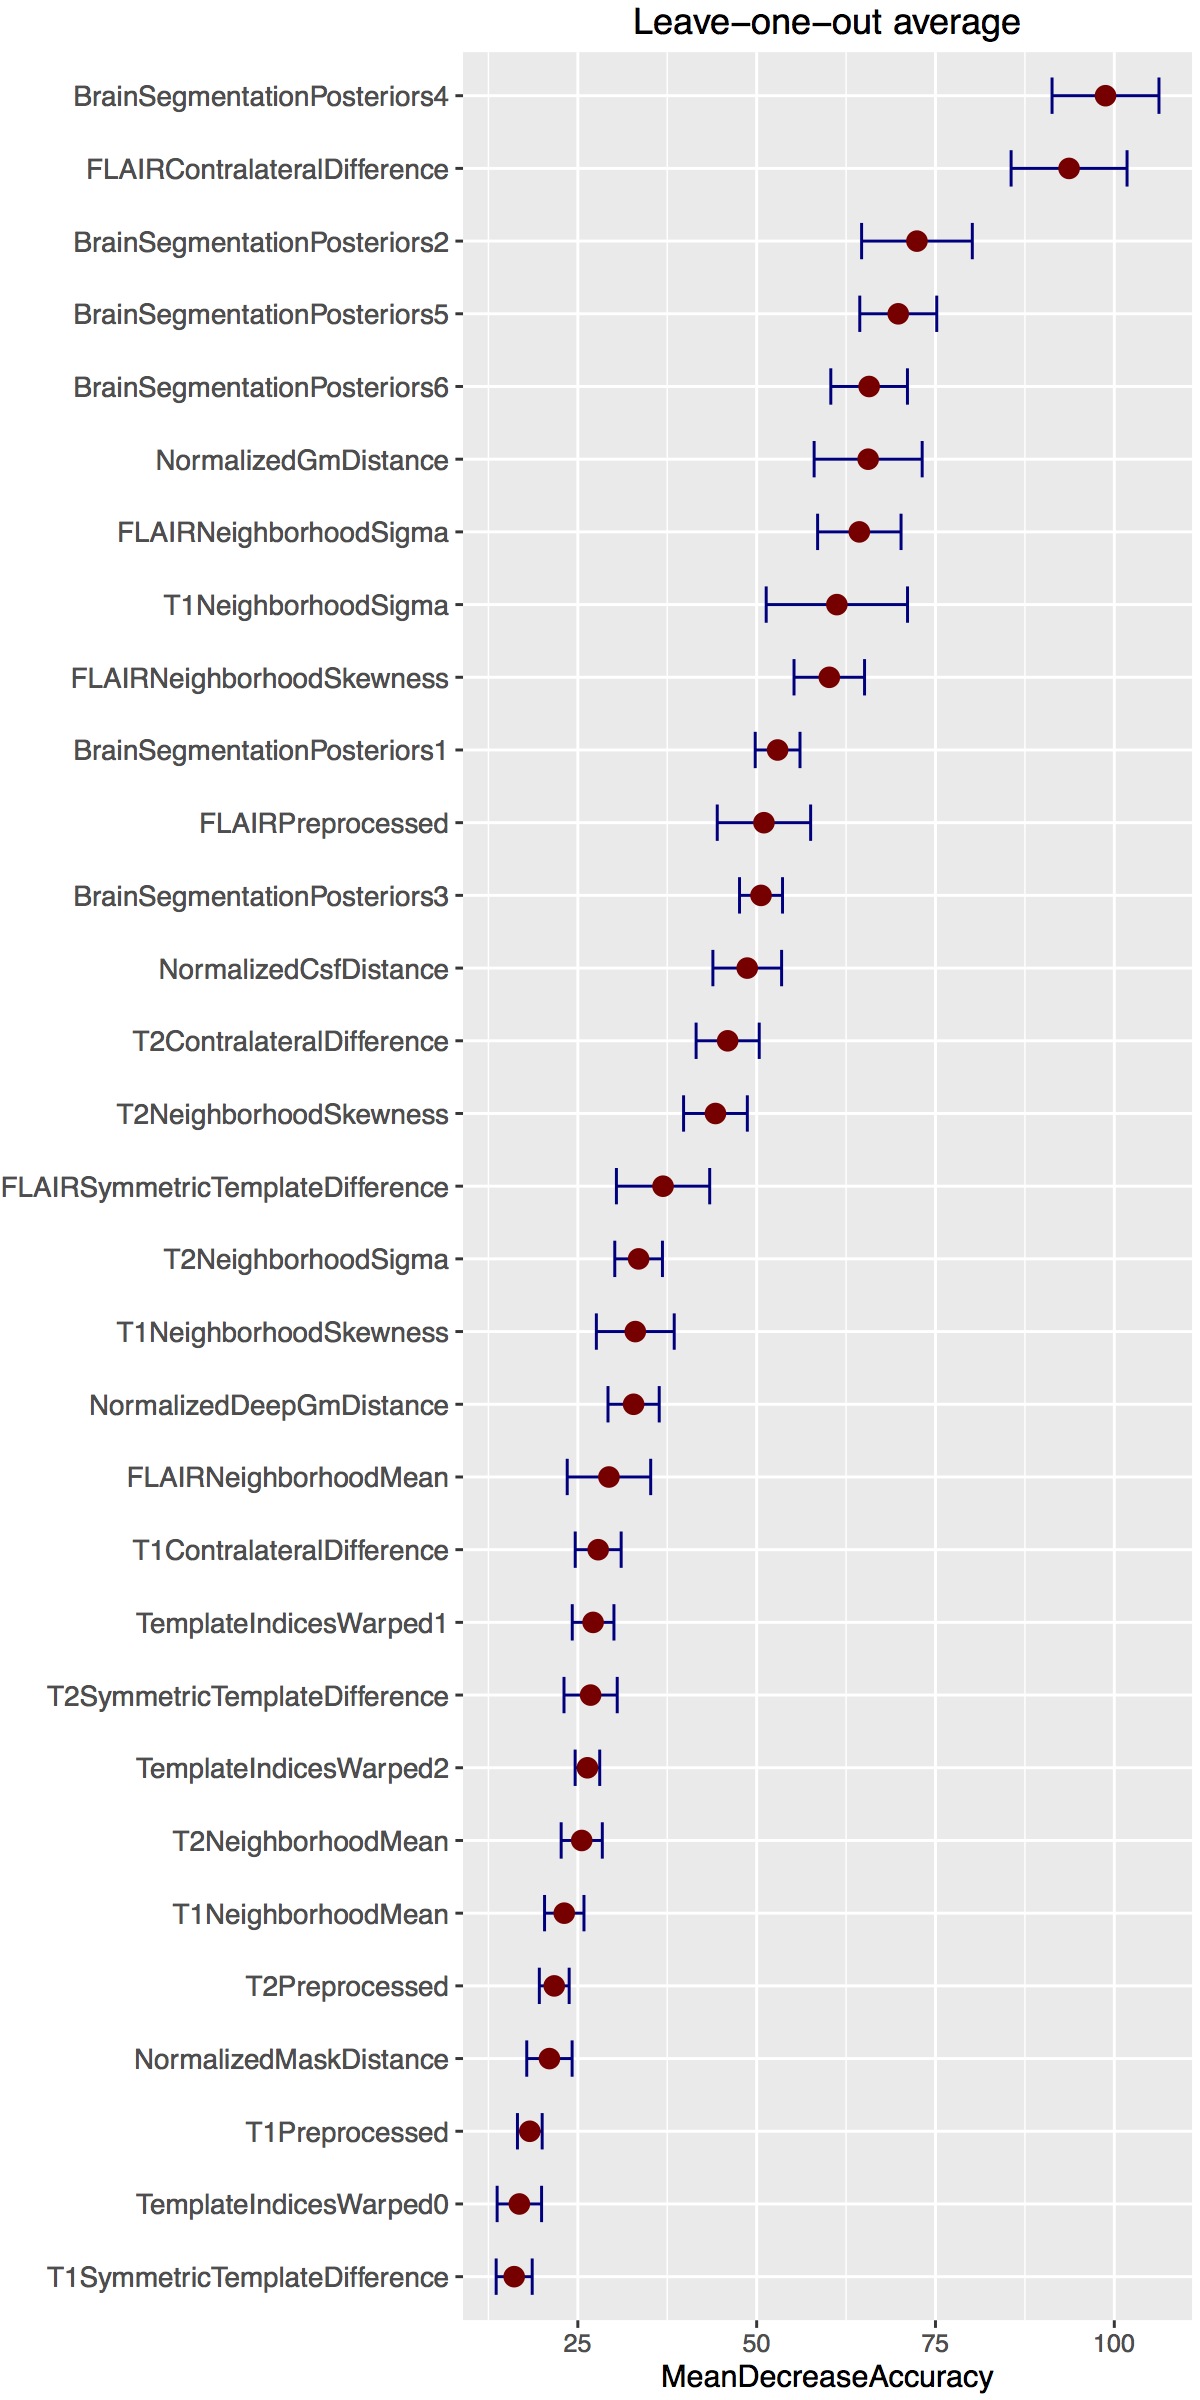
\includegraphics{Figures/averageLeaveOneOutStage1.png}
\caption{Average \texttt{MeanDecreaseAccuracy} plots generated from the
creation of all 24 random forest models for Stage 1 during the
leave-one-out evaluation. These plots are useful in providing a
quantitative assessment of the predictive importance of each feature.
\added[id=nt]{Features are ranked in descending order of importance.}
The horizontal error bars provide the \(95^{th}\) percentile
\deleted[id=bt]{(i.e., $1.96 \times \sigma$)} and illustrate the
stability of the feature importance across the leave-one-out models.
\added[id=nt]{At this initial stage only 31 features images are used.}}
\end{figure}

\begin{figure}[htbp]
\centering
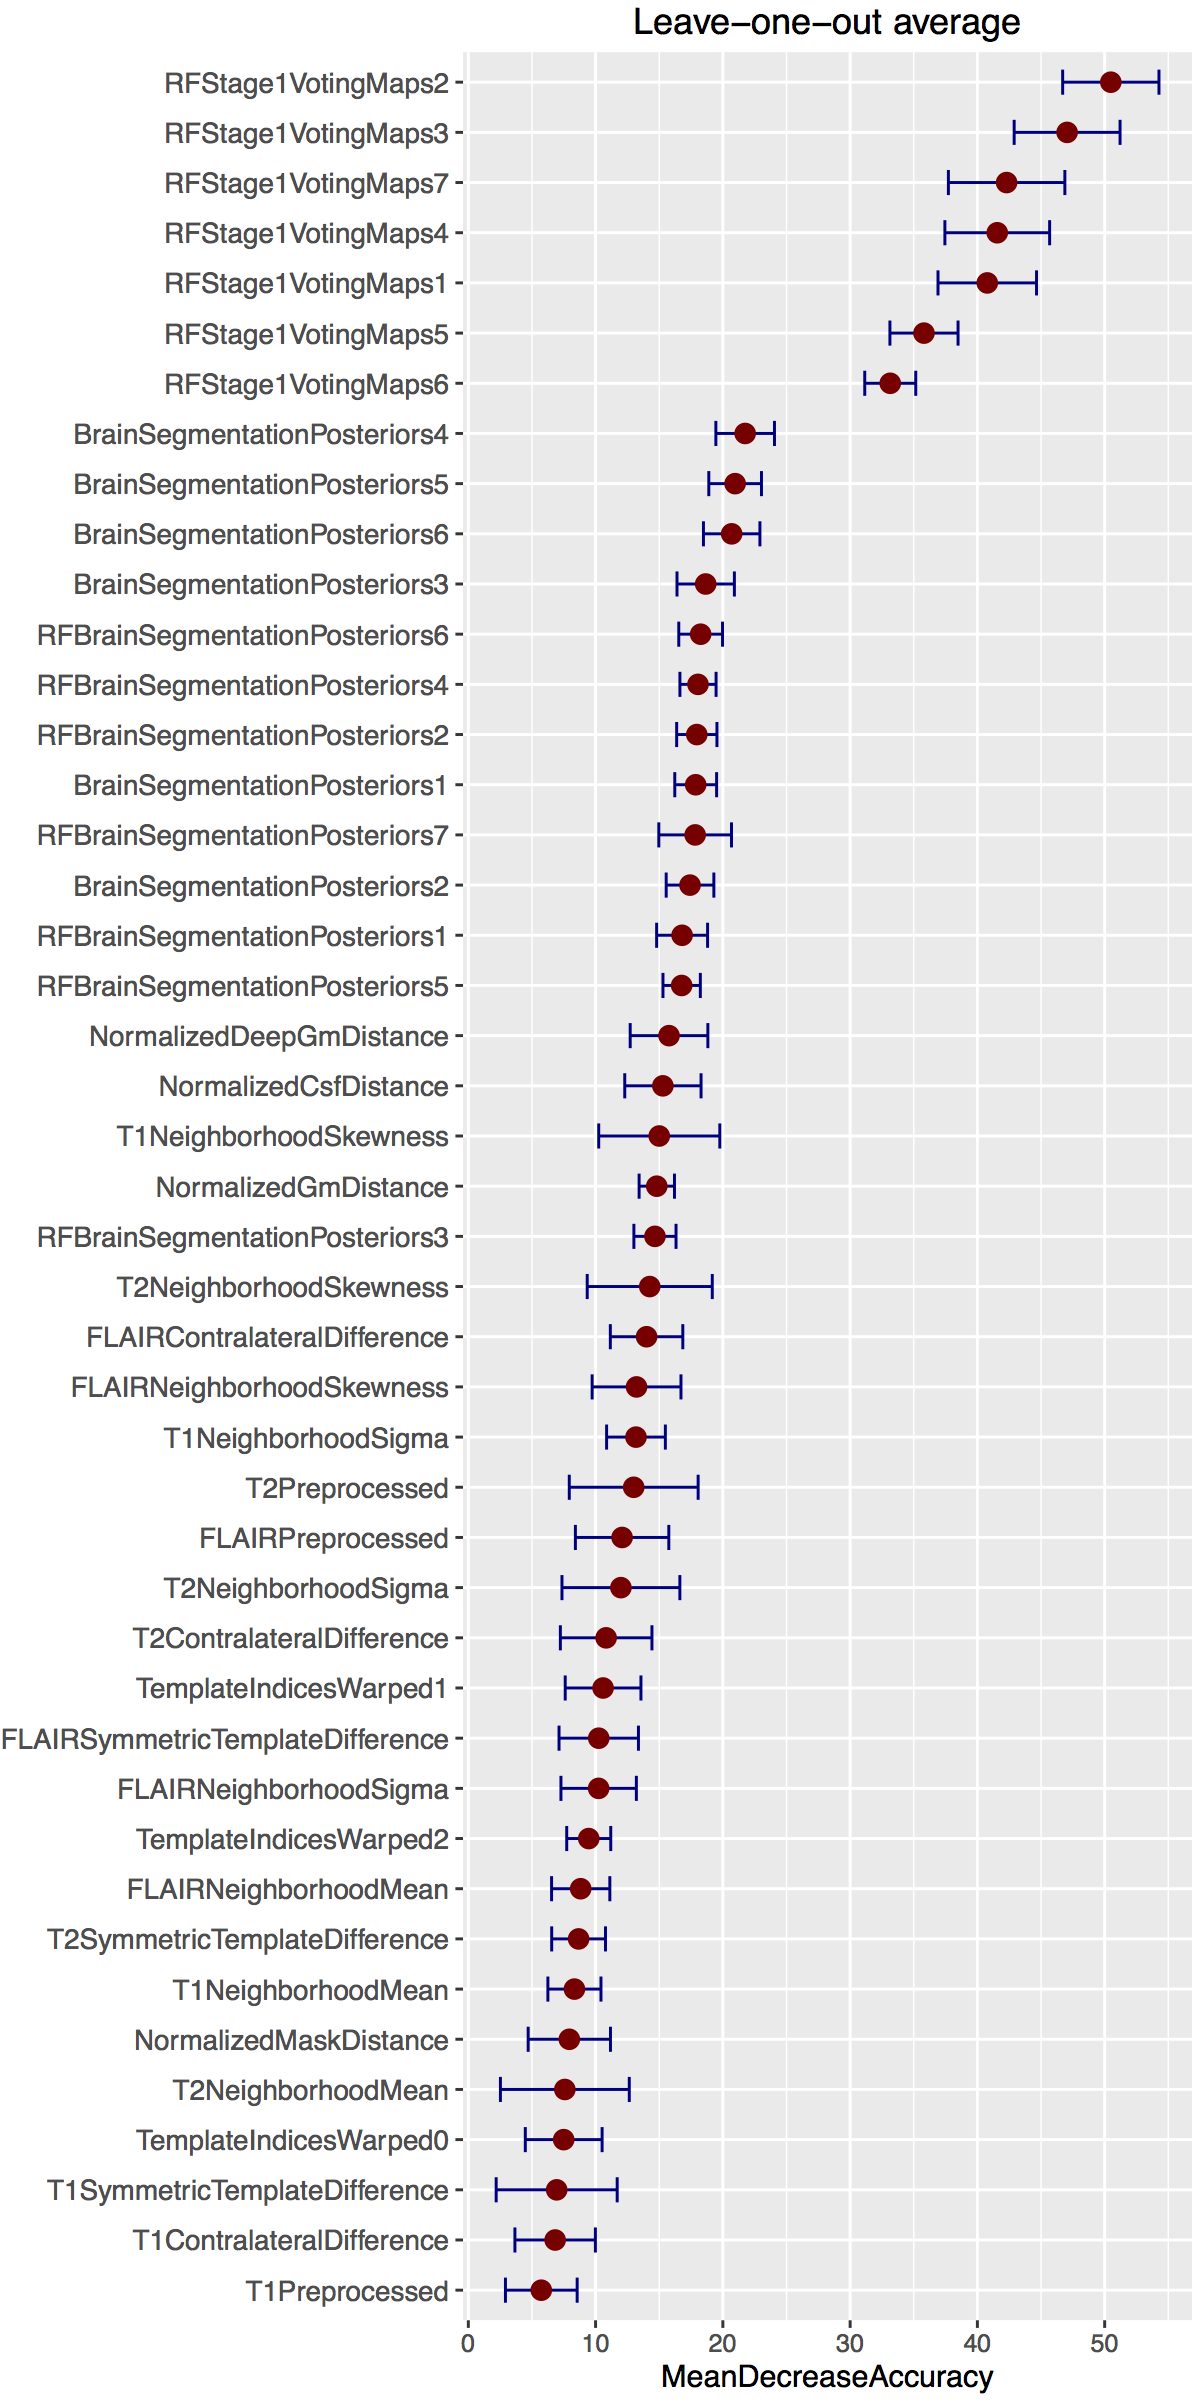
\includegraphics{Figures/averageLeaveOneOutStage2.png}
\caption{Average \texttt{MeanDecreaseAccuracy} plots generated from the
creation of all 24 random forest models for Stage 2 during the
leave-one-out evaluation. These plots are useful in providing a
quantitative assessment of the predictive importance of each feature.
\added[id=nt]{Features are ranked in descending order of importance.}
The horizontal error bars provide the \(95^{th}\) percentile
\deleted[id=bt]{(i.e., $1.96 \times \sigma$)} and illustrate the
stability of the feature importance across the leave-one-out models.
\added[id=nt]{We augment the 31 feature images from the first stage by adding an additional
7 voting maps and 7 segmentation posteriors from application of the Bayesian-based
segmentation for a total of 45 images for the second stage.}}
\end{figure}

The resulting rankings for both Stages are given in Figures 4 and 5
where the values for the separate stages are averaged over the entire
corresponding model set. In addition, we track the variance for each
feature over all models to illustrate the stability of the chosen
features during the evaluation. This latter information is illustrated
as horizontal errors bars providing the \(95^{th}\) percentile
\deleted[id=bt]{(i.e., $1.96 \times \sigma$)}. Note that the reader can
cross reference Table 1 for identifying corresponding feature types and
names.

One can also use these measurements as a type of sanity check. For
example, from the Stage 1 plot, one can see that the
\texttt{MeanDecreaseAccuracy} values for the location indices in the
anterior-posterior direction (i.e., \texttt{TemplateIndicesWarped1}) are
greater than those for either the inferior-superior (i.e.,
\texttt{TemplateIndicesWarped0}) or the left-right (i.e.,
\texttt{TemplateIndicesWarped0}) directions in the space of the
symmetric template.
\deleted[id=bt]{This is intuitive since, as discussed previously, manifestation of TBI white
matter hyperintensities can often be confused with higher intensities at the
periventricular caps in normal subjects [@Neema:2009aa]}
\deleted[id=am]{whereas there does not seem to
be contralateral bias in manifestation of white matter hyperintensities in TBI.}

Additionally, it is interesting to note some of the other top performing
features for Stage 1. The contralateral difference FLAIR image is highly
discriminative over the set of evaluation random forest models
\added[id=bt]{(see Figure 6)}. This accords with the known clinical
relevance of FLAIR images for identifying white matter hyperintensities
and the fact that such pathology does not \added[id=nt]{typically}
manifest symmetrically in both hemispheres. Interestingly, the posterior
maps for the deep gray matter are extremely important for accurate white
matter hyperintensity segmentation. Perhaps the spatial specification of
deep gray matter aids in the removal of false positives. Inspection of
the bottom of the plots demonstrates the lack of discriminating features
associated with the T1 image which is also well-known in the clinical
literature.

\begin{figure}[htbp]
\centering
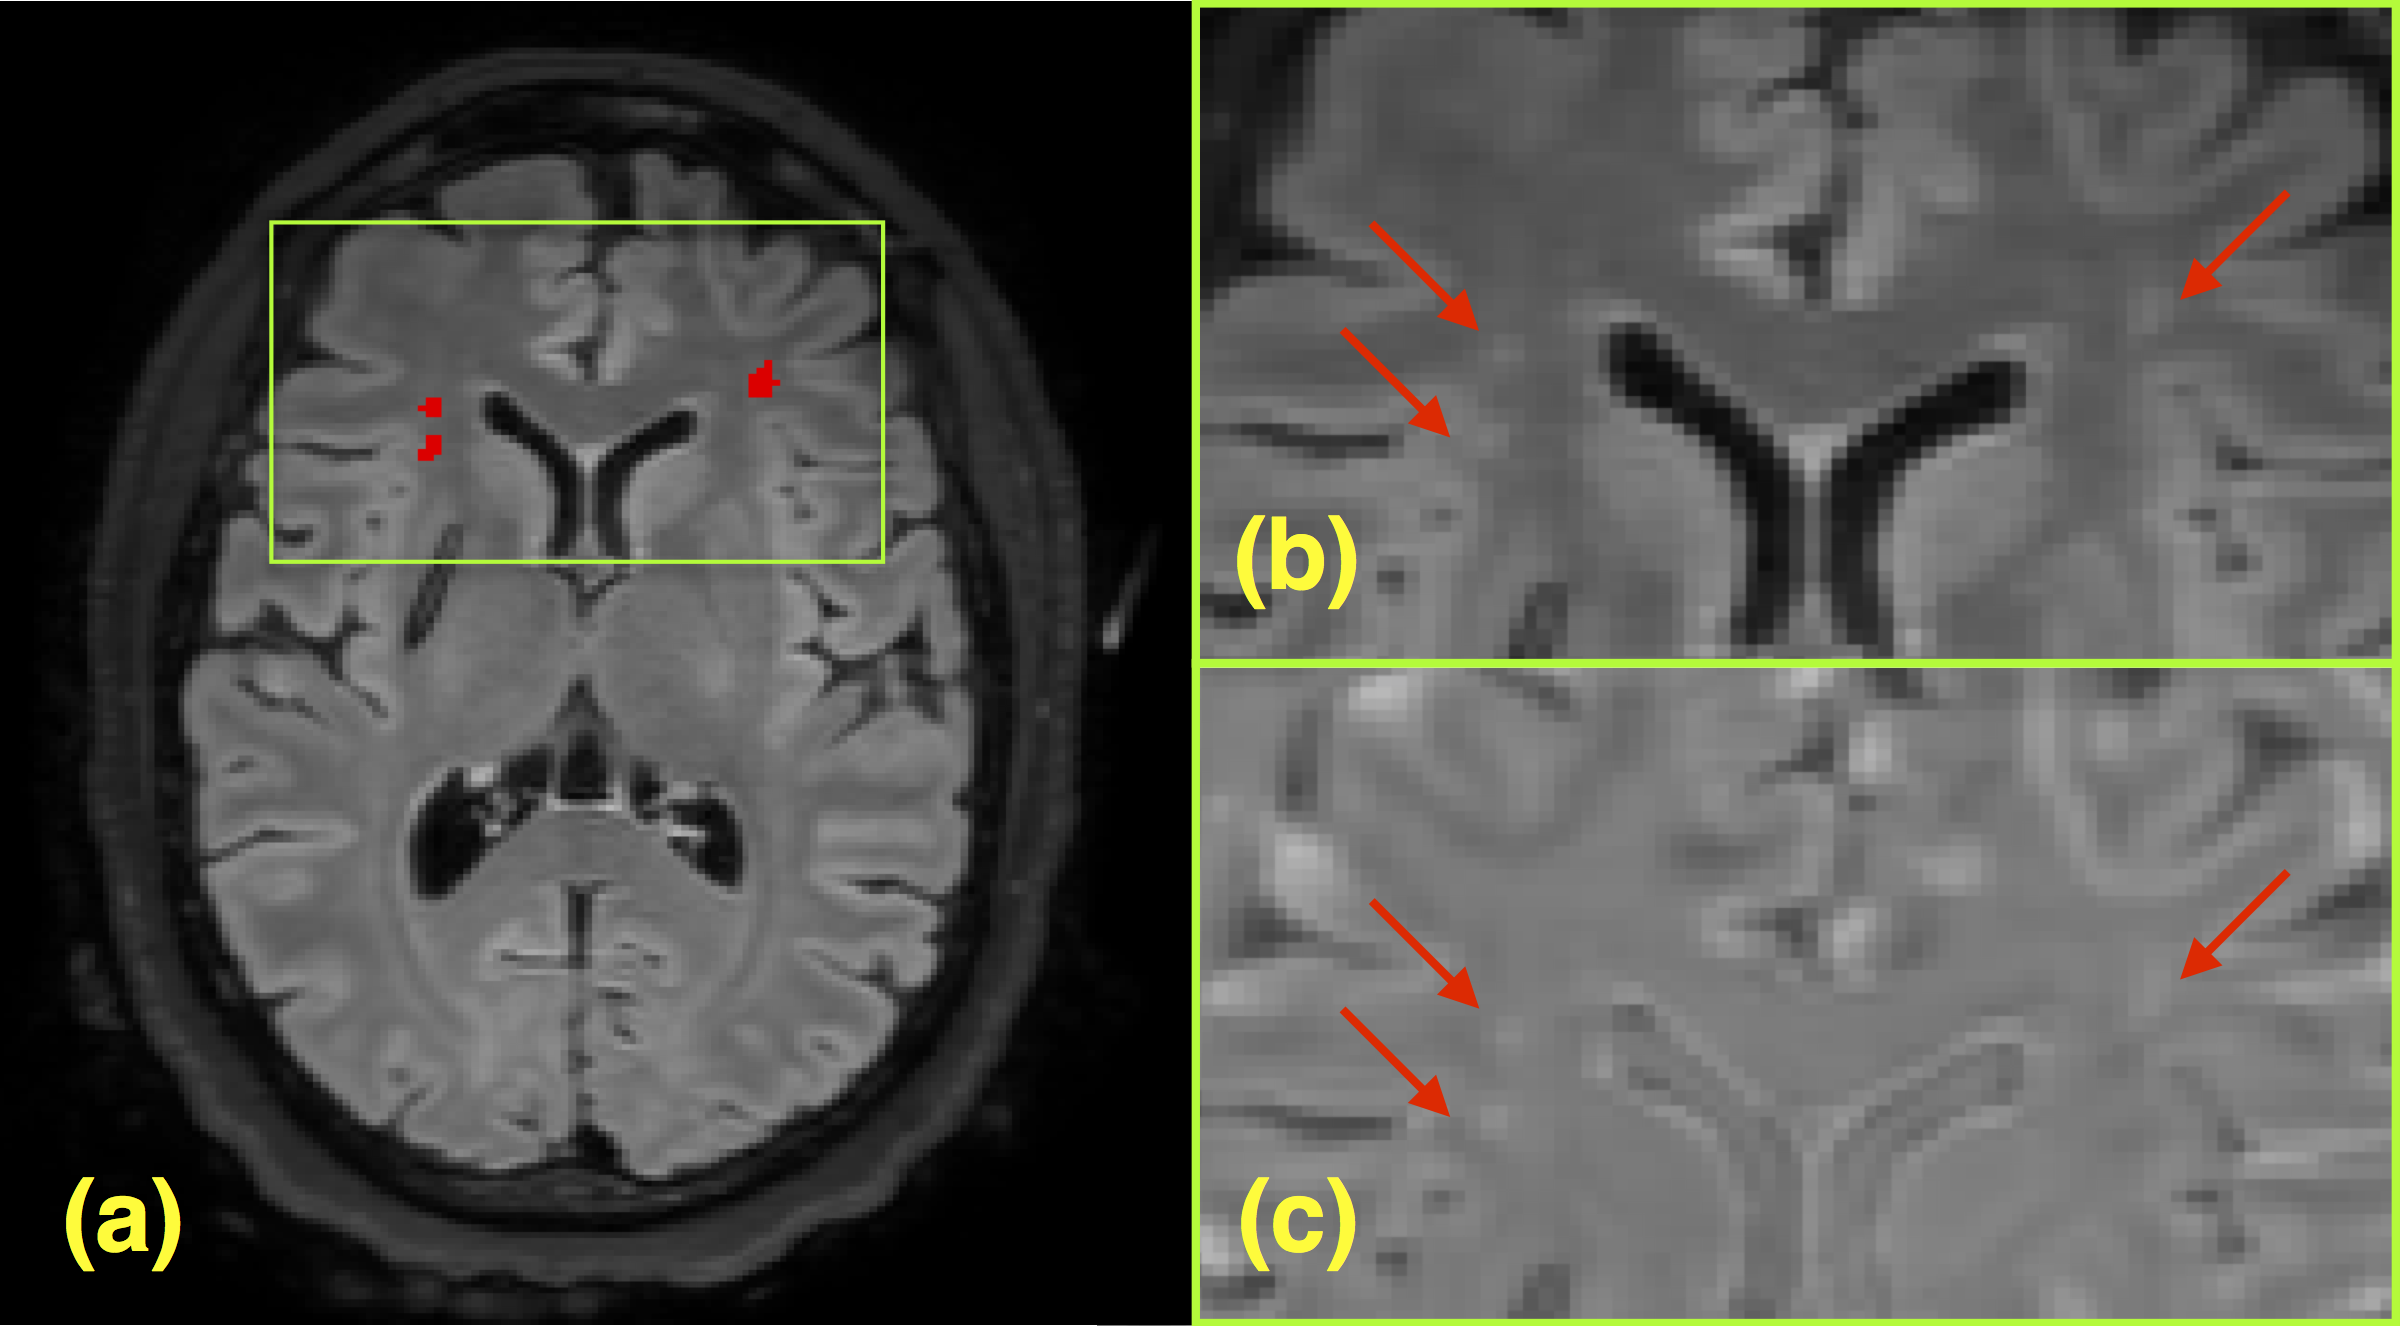
\includegraphics{Figures/FLAIRcontralaleteralWithLesionsAlternate.png}
\caption{\added[id=nt]{(a) FLAIR image slice illustrating WMHs which have been manually delineated.
The region around the WMHs is enlarged (b) in the original FLAIR and the
(c) contralateral FLAIR difference image.}}
\end{figure}

As described earlier, for Stage 2, we used the output random forest
voting maps from Stage 1 as both features themselves and as priors for
input to a Bayesian-based segmentation with an additional MRF spatial
prior. In Figure 5, the voting maps are labeled as
``\texttt{RFStage1VotingMaps}'' where the final numeral is associated
with the brain parenchymal labeling given previously. Similarly, the
additional RF prior segmentation feature probability maps are labeled as
``\texttt{RFBrainSegmentationPosteriors}''. The Stage 2 feature
importance plot follows similar trends as that for Stage 1 with the T1
images not contributing much to the identification of white matter
hyperintensity voxels. The initial voting maps from Stage 1 are
extremely important with the top 3 being the estimated locations of the
1) gray matter, 2) white matter, and 3) white matter hyperintensities.
Since these tissue type can be conflated based on intensity alone it is
intuitive that such features would be important.

\subsection{White matter hyperintensity segmentation
evaluation}\label{white-matter-hyperintensity-segmentation-evaluation}

In Figure 7 are the segmentation comparisons derived from manual
segmentations of the same data. Despite the large variability
characteristic with manual labelings in related
fields\textsuperscript{45,47,48}, such labelings are characteristic of
current clinical practices and the methodology proposed herein is
readily adapted to refinements in training data. On the left of Figure 7
are the improvement in Dice values\textsuperscript{49},
\added[id=nt]{i.e.,}

\[ Dice = 2 \frac{\sum_r|S_r \cap T_r|}{\sum_r|S_r| + |T_r] } \]

\added[id=nt]{over all white matter hyperintensities when comparing the segmentations between the two stages
where the sum is taken over all individually labeled manual, $T_r$, and automated, $S_r$, lesions and $\cap$
represents the intersection between the manual/automated lesion pair.}
Performing the second round of supervised learning improves these Dice
values. One can also note from the right side of Figure 6 that the total
lesion load volume illustrates a few subjects that are severe outliers
in terms of the number of false positives. The second round helps to
correct this issue.

\begin{figure}[htbp]
\centering
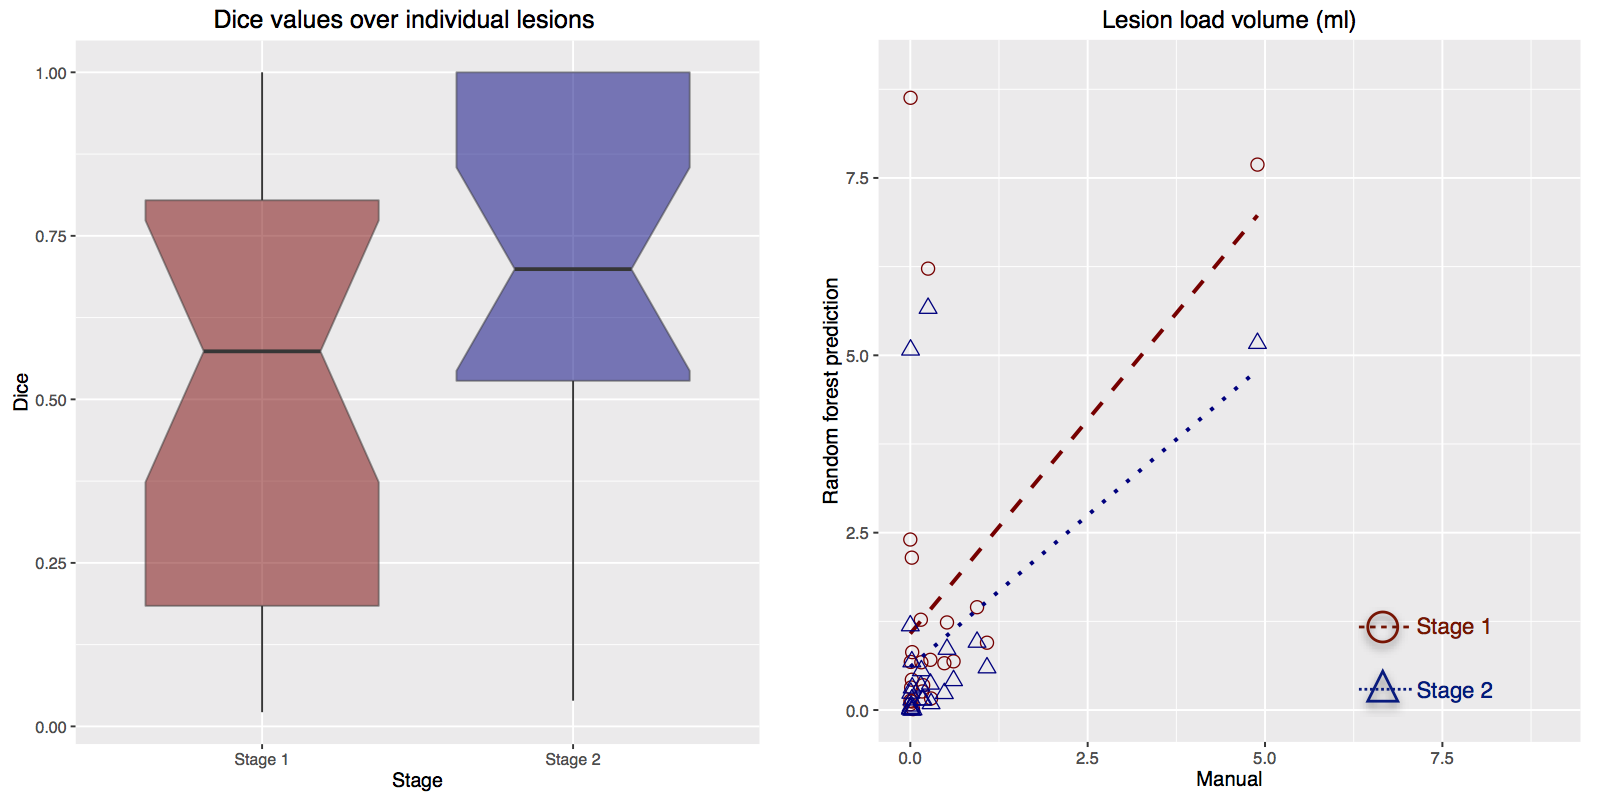
\includegraphics{Figures/llvAndDice.png}
\caption{\added[id=am]{Voxelwise} comparison with manual delineation of
white matter hyperintensities. On the left are the
calculate\added[id=am]{d} Dice values over all white matter
hyperintensities. Note the improvement in the Dice metric from the
employment of the Stage 2 component of the processing pipeline. (Right)
Similar results can be seen by comparing the total lesion load volume
between manual and automated detection strategies. Although some
outliers are found after the Stage 2 processing in a couple subjects,
the number of outliers caused by false positives is
\added[id=lw]{decreased} significantly with the second stage
processing.}
\end{figure}

\section{Discussion}\label{discussion}

\section{}\label{section}

The current communications describes a supervised statistical learning
methodology for identifying WHMs within multimodal MR brain imaging.
This effort utilized information acquired from the manual segmentation
of WMHs from FLAIR images to help build two-stage ensembles of decision
trees for the automated identification of these lesions. Although only a
single expert was used to produce the manual labelings, our intent is to
further refine the proposed paradigm by crowdsourcing with feedback from
other experts who interact with both the data and methodology. Also, we
recognize that only a single site was used for evaluating the proposed
framework. However, we are currently processing other site data with the
models developed for this work and the results look promising since the
developed features are site-agnostic.

As far as we know, this is the first report utilizing a novel random
forest approach to identify WMHs in a cohort of TBI patients. TBI WMHs
tend to be more difficult to segment than MS lesions as the former tend
to be smaller with an overall smaller lesion load. Also, enhancement
protocols with the former tend to be less successful than with the
latter. As mentioned previously, the work in MS lesion segmentation is
extensive with a handful of techniques being publicly available. Our
framework is also available as open-source as part of well-known
neuroimaging tools which easily allows for additions/extensions but is
also, as far as we know, the first random forest-based technique
available for such application.

Two major meta-analyses of WMHs have been published covering the periods
prior to 2010\textsuperscript{9} and after\textsuperscript{10}. The
earlier meta-analysis covered 53 longitudinal studies that included
samples of high-risk populations, i.e., patients selected for a specific
disease or condition such as hypertension, whereas other studies
recruited samples of the general population. Longitudinal studies of
samples representative of the general population are more relevant to
the focus of the present paper. Debette \& Markus\textsuperscript{9}
found that the presence of WMHs was related to subsequent cognitive
decline, a higher risk of developing dementia, stroke, and of mortality.
Lesion volume at baseline was also predictive of cognitive decline.
Limitations of this meta-analysis include heterogeneity in the method of
measuring WMHs; some studies used automated volumetric measurement,
whereas others used a visual rating scale. The studies analyzed by
Debette \& Markus were limited to the occurrence of one of the
aforementioned conditions which they analyzed by hazard ratios.

\replaced[id=dt]{The more}{A} recent meta-analysis by Kloppenborg et
al.\textsuperscript{10} of 23 cross-sectional studies reporting MRI and
concurrent neuropsychological results in patients with heterogeneous
diagnoses but without previously diagnosed cognitive impairment, found
that WMHs were associated with cognitive deficit (effect size of -0.10,
95\% CI: -0.13 to -0.08) after controlling for age. These studies also
differed in the metric used to measure the WMHs, including volume, \% of
total intracranial volume, and a visual rating score. The effect size
for the association with cognitive deficit in these cross-sectional
studies did not differ significantly across various cognitive domains or
the method of measuring lesion volume. Among eight longitudinal studies
analyzed by Kloppenborg et al that included a follow-up MRI and also
controlled for age, the effect size for the association of progression
in WMHs and cognitive impairment was -0.16 (95\% CI:-0.27 to -0.09).
This association was stronger for attention and executive function than
for memory and processing speed. Although baseline WMHs were predictive
of cognitive deficit at follow-up in the seven studies which did not
repeat MRI, the effect size was smaller {[}-0.10 (95\% CI: 0.13 to
-0.05) than in the longitudinal studies that calculated progression in
WMHs. In summary, progression of WMHs seen on repeat MRI has a stronger
relation to cognitive deficit than concurrent imaging findings. These
meta-analyses support the rationale for repeating an MRI in patients
younger than 50 years whose initial scan shows WMHs.

Despite the above-described associations between WMHs, cognitive
decline, increased risk of developing dementia, and mortality, these
lesions receive little attention in current clinical workflows. When
reported in a standard neuroradiologist interpretation, they are
typically handled as incidental findings and are assigned little
clinical significance. This likely reflects the impracticality of
performing a detailed assessment of number, volume, and distribution
within a qualitative neuroradiologist interpretation as well as the lack
of correlative information on how the presence and distribution of these
lesions may inform a diagnosis and prognosis in the appropriate clinical
setting. To date, automated or semi-automated tools for the detection of
WMHs have lacked the specificity and efficiency for the mining of
large-scale datasets to generate highly granular data on whether these
lesions possess any true diagnostic or prognostic value in the setting
of a specific disease process. The present communication describes a
supervised statistical learning tool that is appropriate for the
application to such large-scale datasets.

The currently described tool is just one example of how ``supervised
learning'' algorithms might be applied to aid in the diagnosis of TBI
and other disease processes through the specific identification of
features predictive of a given disease state. It is an important
demonstration of the potential power of these analytical approaches in
the rapid but comprehensive mining of information from neuroimaging
examinations. Supervised learning algorithms are presently employed
across a wide variety of settings for the rapid identification of
predictive imaging features\textsuperscript{50--53}. Automobile
manufacturers utilize these types of approaches to equip self-driving
vehicles to recognize and respond to unique external surroundings
through the identification of visual information sufficiently similar to
previously assimilated training data\textsuperscript{54,55}. Similarly,
in the context of the neuroimaging assessments, deep learning approaches
may allow for the rapid identification of information predictive of
disease state in an individual patient. These approaches have been
applied to the segmentation of macroscopically visible
structures\textsuperscript{50--53}. Additionally, these approaches might
be applied to the interrogation of imaging data in the individual
patient with a primary quantitative output metrics to include sequences
such as diffusion tensor imaging (DTI) and its variants, functional
connectivity, perfusion weighted imaging, and cortical thickness
assessments. At present, these advanced neuroimaging sequences are
confined to cohort-based research studies due to the lack of available
analytical tools to assess the information in the setting of the
individual patient\textsuperscript{56}. Application of deep learning
approaches in the context of data with primary quantitative outputs will
require large scale normative and disease specific databases. Building
these large scale imaging libraries is resource intensive and requires a
multi-center approach with harmonized scanners between sites and
correlative non-imaging clinical data. Large scale TBI data is becoming
increasingly available through activities such as the Chronic Effects of
Neurotrauma Consortium (CENC), Transforming Research and Clinical
Knowledge in TBI (TRACK-TBI), Collaborative European Neurotrauma
Effectiveness Research in TBI (CENTER-TBI), Department of Defense
Alzheimer's Disease Neuroimaging Initiative (DOD-ADNI), and other data
being consolidated through FITBIR. In concert with any available high
quality normative neuroimaging data, deep learning algorithms may be
well positioned to help transform how neuroimaging is interpreted for
the clinical management of patients with this disease process.

\clearpage

\section*{References}\label{references}
\addcontentsline{toc}{section}{References}

\hypertarget{refs}{}
\hypertarget{ref-Bigler:2013aa}{}
1. Bigler ED, Abildskov TJ, Petrie J, Farrer TJ, Dennis M, Simic N,
Taylor HG, Rubin KH, Vannatta K, Gerhardt CA, et al. Heterogeneity of
brain lesions in pediatric traumatic brain injury. Neuropsychology.
2013;27(4):438--51.

\hypertarget{ref-Smitherman:2016aa}{}
2. Smitherman E, Hernandez A, Stavinoha PL, Huang R, Kernie SG,
Diaz-Arrastia R, Miles DK. Predicting outcome after pediatric traumatic
brain injury by early magnetic resonance imaging lesion location and
volume. J Neurotrauma. 2016;33(1):35--48.

\hypertarget{ref-Marquez-de-la-Plata:2007aa}{}
3. Marquez de la Plata C, Ardelean A, Koovakkattu D, Srinivasan P,
Miller A, Phuong V, Harper C, Moore C, Whittemore A, Madden C, et al.
Magnetic resonance imaging of diffuse axonal injury: Quantitative
assessment of white matter lesion volume. J Neurotrauma.
2007;24(4):591--8.

\hypertarget{ref-Moen:2014aa}{}
4. Moen KG, Brezova V, Skandsen T, Håberg AK, Folvik M, Vik A. Traumatic
axonal injury: The prognostic value of lesion load in corpus callosum,
brain stem, and thalamus in different magnetic resonance imaging
sequences. J Neurotrauma. 2014;31(17):1486--96.

\hypertarget{ref-Ding:2008aa}{}
5. Ding K, Marquez de la Plata C, Wang JY, Mumphrey M, Moore C, Harper
C, Madden CJ, McColl R, Whittemore A, Devous MD, et al. Cerebral atrophy
after traumatic white matter injury: Correlation with acute neuroimaging
and outcome. J Neurotrauma. 2008;25(12):1433--40.

\hypertarget{ref-Pierallini:2000aa}{}
6. Pierallini A, Pantano P, Fantozzi LM, Bonamini M, Vichi R, Zylberman
R, Pisarri F, Colonnese C, Bozzao L. Correlation between mRI findings
and long-term outcome in patients with severe brain trauma.
Neuroradiology. 2000;42(12):860--7.

\hypertarget{ref-Weiss:2008aa}{}
7. Weiss N, Galanaud D, Carpentier A, Tezenas de Montcel S, Naccache L,
Coriat P, Puybasset L. A combined clinical and mRI approach for outcome
assessment of traumatic head injured comatose patients. J Neurol.
2008;255(2):217--23.

\hypertarget{ref-Levin:1988aa}{}
8. Levin HS, Williams D, Crofford MJ, High WM Jr, Eisenberg HM, Amparo
EG, Guinto FC Jr, Kalisky Z, Handel SF, Goldman AM. Relationship of
depth of brain lesions to consciousness and outcome after closed head
injury. J Neurosurg. 1988;69(6):861--6.

\hypertarget{ref-Debette:2010aa}{}
9. Debette S, Markus HS. The clinical importance of white matter
hyperintensities on brain magnetic resonance imaging: Systematic review
and meta-analysis. BMJ. 2010;341:c3666.

\hypertarget{ref-Kloppenborg:2014aa}{}
10. Kloppenborg RP, Nederkoorn PJ, Geerlings MI, Berg E van den.
Presence and progression of white matter hyperintensities and cognition:
A meta-analysis. Neurology. 2014;82(23):2127--38.

\hypertarget{ref-mlmi2015}{}
11.

\hypertarget{ref-Bauer:2011aa}{}
12. Bauer S, Nolte L-P, Reyes M. Fully automatic segmentation of brain
tumor images using support vector machine classification in combination
with hierarchical conditional random field regularization. Med Image
Comput Comput Assist Interv. 2011;14(Pt 3):354--61.

\hypertarget{ref-Tong:2014aa}{}
13. Tong T, Wolz R, Gao Q, Guerrero R, Hajnal JV, Rueckert D,
Alzheimer's Disease Neuroimaging Initiative. Multiple instance learning
for classification of dementia in brain mRI. Med Image Anal.
2014;18(5):808--18.

\hypertarget{ref-Liu:2013aa}{}
14. Liu X, Tosun D, Weiner MW, Schuff N, Alzheimer's Disease
Neuroimaging Initiative. Locally linear embedding (lLE) for mRI based
alzheimer's disease classification. Neuroimage. 2013;83:148--57.

\hypertarget{ref-Van-Horn:2014aa}{}
15. Van Horn JD, Toga AW. Human neuroimaging as a ``big data'' science.
Brain Imaging Behav. 2014;8(2):323--31.

\hypertarget{ref-scipy}{}
16. Jones E, Oliphant T, Peterson P, others. SciPy: Open source
scientific tools for Python. 2001--2001-\/-.

\hypertarget{ref-R}{}
17. R Core Team. R: A Language and Environment for Statistical
Computing. Vienna, Austria: R Foundation for Statistical Computing;
2016.

\hypertarget{ref-breiman2001}{}
18. Breiman L. Random forests. In: Machine learning. 2001. pp. 5--32.

\hypertarget{ref-yi2009}{}
19. Yi Z, Criminisi A, Shotton J, Blake A. Discriminative, semantic
segmentation of brain tissue in MR images. Med Image Comput Comput
Assist Interv. 2009;12(Pt 2):558--65.

\hypertarget{ref-viola2005}{}
20. Viola P, Jones M, Snow D. Detecting pedestrians using patterns of
motion and appearance. International Journal of Computer Vision.
2005;63:153--161.

\hypertarget{ref-geremia2011}{}
21. Geremia E, Clatz O, Menze BH, Konukoglu E, Criminisi A, Ayache N.
Spatial decision forests for MS lesion segmentation in multi-channel
magnetic resonance images. Neuroimage. 2011;57(2):378--90.

\hypertarget{ref-Pustina:2016aa}{}
22. Pustina D, Coslett HB, Turkeltaub PE, Tustison N, Schwartz MF,
Avants B. Automated segmentation of chronic stroke lesions using lINDA:
Lesion identification with neighborhood data analysis. Hum Brain Mapp.
2016 Jan.

\hypertarget{ref-geremia2012}{}
23. Geremia E, Menze BH, Ayache N. Spatial decision forests for glioma
segmentation in multi-channel MR images. In: Proceedings of MICCAI-BRATS
2012. 2012.

\hypertarget{ref-bauer2012}{}
24. Bauer S, Fejes T, Slotboom J, Wiest R, Nolte L-P, Reyes M.
Segmentation of brain tumor images based on integrated hierarchical
classification and regularization. In: Proceedings of MICCAI-BRATS 2012.
2012. pp. 10--13.

\hypertarget{ref-zikic2012}{}
25. Zikic D, Glocker B, Konukoglu E, Shotton J, Criminisi A, Ye DH,
Demiralp C, Thomas OM, Das T, Jena R, et al. Context-sensitive
classification forests for segmentation of brain tumor tissues. In:
Proceedings of MICCAI-BRATS 2012. 2012. pp. 1--9.

\hypertarget{ref-Tustison:2015aa}{}
26. Tustison NJ, Shrinidhi KL, Wintermark M, Durst CR, Kandel BM, Gee
JC, Grossman MC, Avants BB. Optimal symmetric multimodal templates and
concatenated random forests for supervised brain tumor segmentation
(simplified) with aNTsR. Neuroinformatics. 2015;13(2):209--25.

\hypertarget{ref-Menze:2015aa}{}
27. Menze BH, Jakab A, Bauer S, Kalpathy-Cramer J, Farahani K, Kirby J,
Burren Y, Porz N, Slotboom J, Wiest R, et al. The multimodal brain tumor
image segmentation benchmark (bRATS). IEEE Trans Med Imaging.
2015;34(10):1993--2024.

\hypertarget{ref-schapire1990}{}
28. Schapire R. The strength of weak learnability. Machine Learning.
1990;5:197--227.

\hypertarget{ref-freund1997}{}
29. Freund Y, Schapire R. A decision-theoretic generalization of on-line
learning and an application to boosting. Journal of Computer and System
Sciences. 1997;55:119--139.

\hypertarget{ref-ho1995}{}
30. Ho TK. Random decision forests. In: Document analysis and
recognition, 1995., proceedings of the third international conference
on. Vol. 1. 1995. pp. 278--282 vol.1.

\hypertarget{ref-amit1997}{}
31. Amit Y, Geman D. Shape quantization and recognition with randomized
trees. Neural Computation. 1997;9:1545--1588.

\hypertarget{ref-Neema:2009aa}{}
32. Neema M, Guss ZD, Stankiewicz JM, Arora A, Healy BC, Bakshi R.
Normal findings on brain fluid-attenuated inversion recovery mR images
at 3T. AJNR Am J Neuroradiol. 2009;30(5):911--6.

\hypertarget{ref-Avants:2014aa}{}
33. Avants BB, Tustison NJ, Stauffer M, Song G, Wu B, Gee JC. The
Insight ToolKit image registration framework. Front Neuroinform.
2014;8:44.

\hypertarget{ref-Tustison:2010ac}{}
34. Tustison NJ, Avants BB, Cook PA, Zheng Y, Egan A, Yushkevich PA, Gee
JC. N4ITK: Improved N3 bias correction. IEEE Trans Med Imaging.
2010;29(6):1310--20.

\hypertarget{ref-Manjon:2010aa}{}
35. Manjón JV, Coupé P, Martí-Bonmatí L, Collins DL, Robles M. Adaptive
non-local means denoising of mR images with spatially varying noise
levels. J Magn Reson Imaging. 2010;31(1):192--203.

\hypertarget{ref-Tustison:2014ab}{}
36. Tustison NJ, Cook PA, Klein A, Song G, Das SR, Duda JT, Kandel BM,
Strien N van, Stone JR, Gee JC, et al. Large-scale evaluation of aNTs
and freeSurfer cortical thickness measurements. Neuroimage.
2014;99:166--79.

\hypertarget{ref-nyul2000}{}
37. Nyúl LG, Udupa JK, Zhang X. New variants of a method of MRI scale
standardization. IEEE Trans Med Imaging. 2000;19(2):143--50.

\hypertarget{ref-Yushkevich:2006aa}{}
38. Yushkevich PA, Piven J, Hazlett HC, Smith RG, Ho S, Gee JC, Gerig G.
User-guided 3D active contour segmentation of anatomical structures:
Significantly improved efficiency and reliability. Neuroimage.
2006;31(3):1116--28.

\hypertarget{ref-Avants:2011aa}{}
39. Avants BB, Tustison NJ, Wu J, Cook PA, Gee JC. An open source
multivariate framework for \(n\)-tissue segmentation with evaluation on
public data. Neuroinformatics. 2011;9(4):381--400.

\hypertarget{ref-landman2011}{}
40. Landman BA, Huang AJ, Gifford A, Vikram DS, Lim IAL, Farrell JAD,
Bogovic JA, Hua J, Chen M, Jarso S, et al. Multi-parametric neuroimaging
reproducibility: A 3-T resource study. Neuroimage. 2011;54(4):2854--66.

\hypertarget{ref-maurer2003}{}
41. Maurer CR, Rensheng Q, Raghavan V. A linear time algorithm for
computing exact Euclidean distance transforms of binary images in
arbitrary dimensions. Pattern Analysis and Machine Intelligence, IEEE
Transactions on. 2003;25(2):265--270.

\hypertarget{ref-Tustison:2013ac}{}
42. Tustison NJ, Avants BB. Explicit B-spline regularization in
diffeomorphic image registration. Front Neuroinform. 2013;7:39.

\hypertarget{ref-Avants:2011ab}{}
43. Avants BB, Tustison NJ, Song G, Cook PA, Klein A, Gee JC. A
reproducible evaluation of ANTs similarity metric performance in brain
image registration. Neuroimage. 2011;54(3):2033--44.

\hypertarget{ref-Anbeek:2004aa}{}
44. Anbeek P, Vincken KL, Osch MJP van, Bisschops RHC, Grond J van der.
Probabilistic segmentation of white matter lesions in mR imaging.
Neuroimage. 2004;21(3):1037--44.

\hypertarget{ref-Garcia-Lorenzo:2013aa}{}
45. García-Lorenzo D, Francis S, Narayanan S, Arnold DL, Collins DL.
Review of automatic segmentation methods of multiple sclerosis white
matter lesions on conventional magnetic resonance imaging. Med Image
Anal. 2013;17(1):1--18.

\hypertarget{ref-liaw2002}{}
46. Liaw A, Wiener M. Classification and regression by randomForest. R
News. 2002;2/3:18--22.

\hypertarget{ref-Grimaud:1996aa}{}
47. Grimaud J, Lai M, Thorpe J, Adeleine P, Wang L, Barker GJ, Plummer
DL, Tofts PS, McDonald WI, Miller DH. Quantification of mRI lesion load
in multiple sclerosis: A comparison of three computer-assisted
techniques. Magn Reson Imaging. 1996;14(5):495--505.

\hypertarget{ref-styner2008}{}
48. Styner M, Lee J, Chin B, Chin M, Commowick O, Tran H, Markovic-Plese
S, Jewells V, Warfield S, editors. Special Issue on 2008 MICCAI Workshop
- MS Lesion Segmentation. MIDAS J; 2008.

\hypertarget{ref-tustison2009}{}
49. Tustison NJ, Gee JC. Introducing Dice, Jaccard, and other label
overlap measures to ITK. Insight Journal. 2009.

\hypertarget{ref-Plis:2014aa}{}
50. Plis SM, Hjelm DR, Salakhutdinov R, Allen EA, Bockholt HJ, Long JD,
Johnson HJ, Paulsen JS, Turner JA, Calhoun VD. Deep learning for
neuroimaging: A validation study. Front Neurosci. 2014;8:229.

\hypertarget{ref-Suk:2015aa}{}
51. Suk H-I, Lee S-W, Shen D, Alzheimer's Disease Neuroimaging
Initiative. Deep sparse multi-task learning for feature selection in
alzheimer's disease diagnosis. Brain Struct Funct. 2015 May.

\hypertarget{ref-Li:2014aa}{}
52. Li R, Zhang W, Suk H-I, Wang L, Li J, Shen D, Ji S. Deep learning
based imaging data completion for improved brain disease diagnosis. Med
Image Comput Comput Assist Interv. 2014;17(Pt 3):305--12.

\hypertarget{ref-Liu:2015aa}{}
53. Liu S, Liu S, Cai W, Che H, Pujol S, Kikinis R, Feng D, Fulham MJ,
ADNI. Multimodal neuroimaging feature learning for multiclass diagnosis
of alzheimer's disease. IEEE Trans Biomed Eng. 2015;62(4):1132--40.

\hypertarget{ref-HadsellSBESKML09}{}
54. Hadsell R, Sermanet P, Ben J, Erkan A, Scoffier M, Kavukcuoglu K,
Muller U, LeCun Y. Learning long-range vision for autonomous off-road
driving. J. Field Robotics. 2009;26(2):120--144.

\hypertarget{ref-FarabetCNL12}{}
55. Farabet C, Couprie C, Najman L, LeCun Y. Scene parsing with
multiscale feature learning, purity trees, and optimal covers. In:
Proceedings of the 29th international conference on machine learning,
ICML 2012, edinburgh, scotland, uK, june 26 - july 1, 2012. icml.cc /
Omnipress; 2012.

\hypertarget{ref-Mayer:2014aa}{}
56. Mayer AR, Bedrick EJ, Ling JM, Toulouse T, Dodd A. Methods for
identifying subject-specific abnormalities in neuroimaging data. Hum
Brain Mapp. 2014;35(11):5457--70.

\end{document}
